\newpage
\section{RESULTS AND DISCUSSION}

%%%%%%%%%%%%%%%%%%%%%%%%%%%%%%%%%%%%%%%%%%%%%%%%%%%%%%%%%%%%%%%%%%%%%%%%%%%%%%%%%%%%%%%%
%%%%%%%%%%%%%%%%%%%%%%%%%%%%%%%%%%%%%%%%%%%%%%%%%%%%%%%%%%%%%%%%%%%%%%%%%%%%%%%%%%%%%%%%
The results section is divided into three logical blocks. First, simulations of the neat polymer were performed to verify the force field and to determine the key properties of the polymer. Subsequently, a series of neat API simulations were performed. Then, simulations of mixtures of different API concentrations in polymer were performed to see the behavior of the mixtures.  

\subsection{Simulations of neat PLA}
\subsubsection{Structural properties}
First, the simulations from 2 initial states were done (fibrilar and globular). The Figure \ref{fig:linearni} shows an example of the shortest polymer in a fibrilar conformation state, whereas Figure \ref{fig:sbalene} displays globular conformations of chains containing 20 and 200 monomer units on the left and right, respectively. 

\begin{figure}[htb]
	\centering
	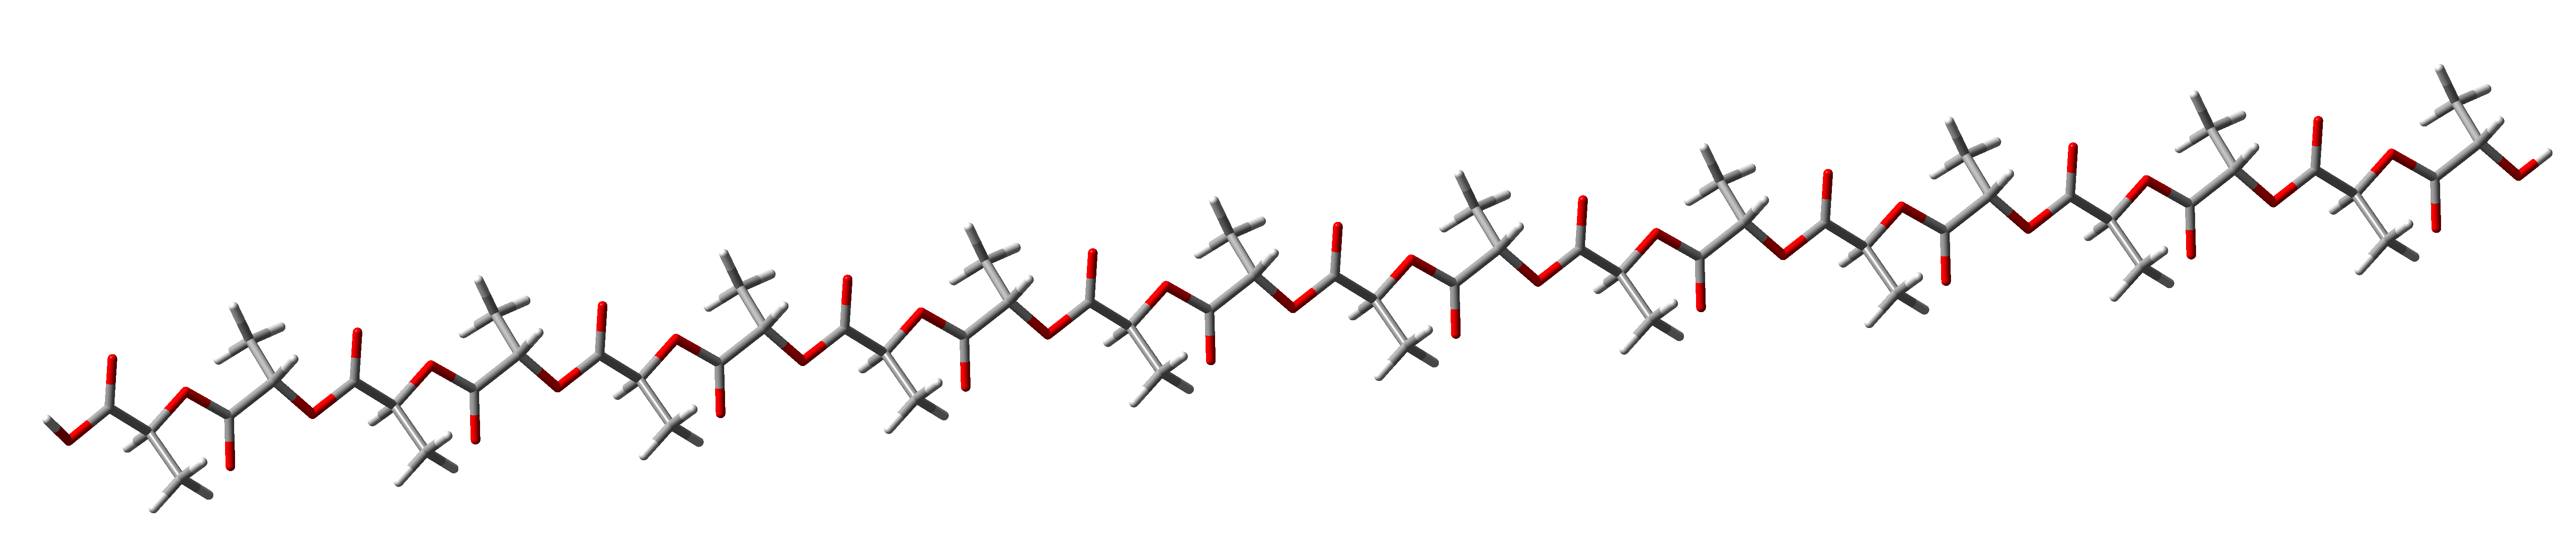
\includegraphics[width=0.9\linewidth]{img/pla_10d_tube.png}
	\caption{Fibrilar PLA polymer chain, 20 units}
	\label{fig:linearni}
\end{figure}

\begin{figure}[htb]
	\begin{subfigure}{0.5\textwidth}
		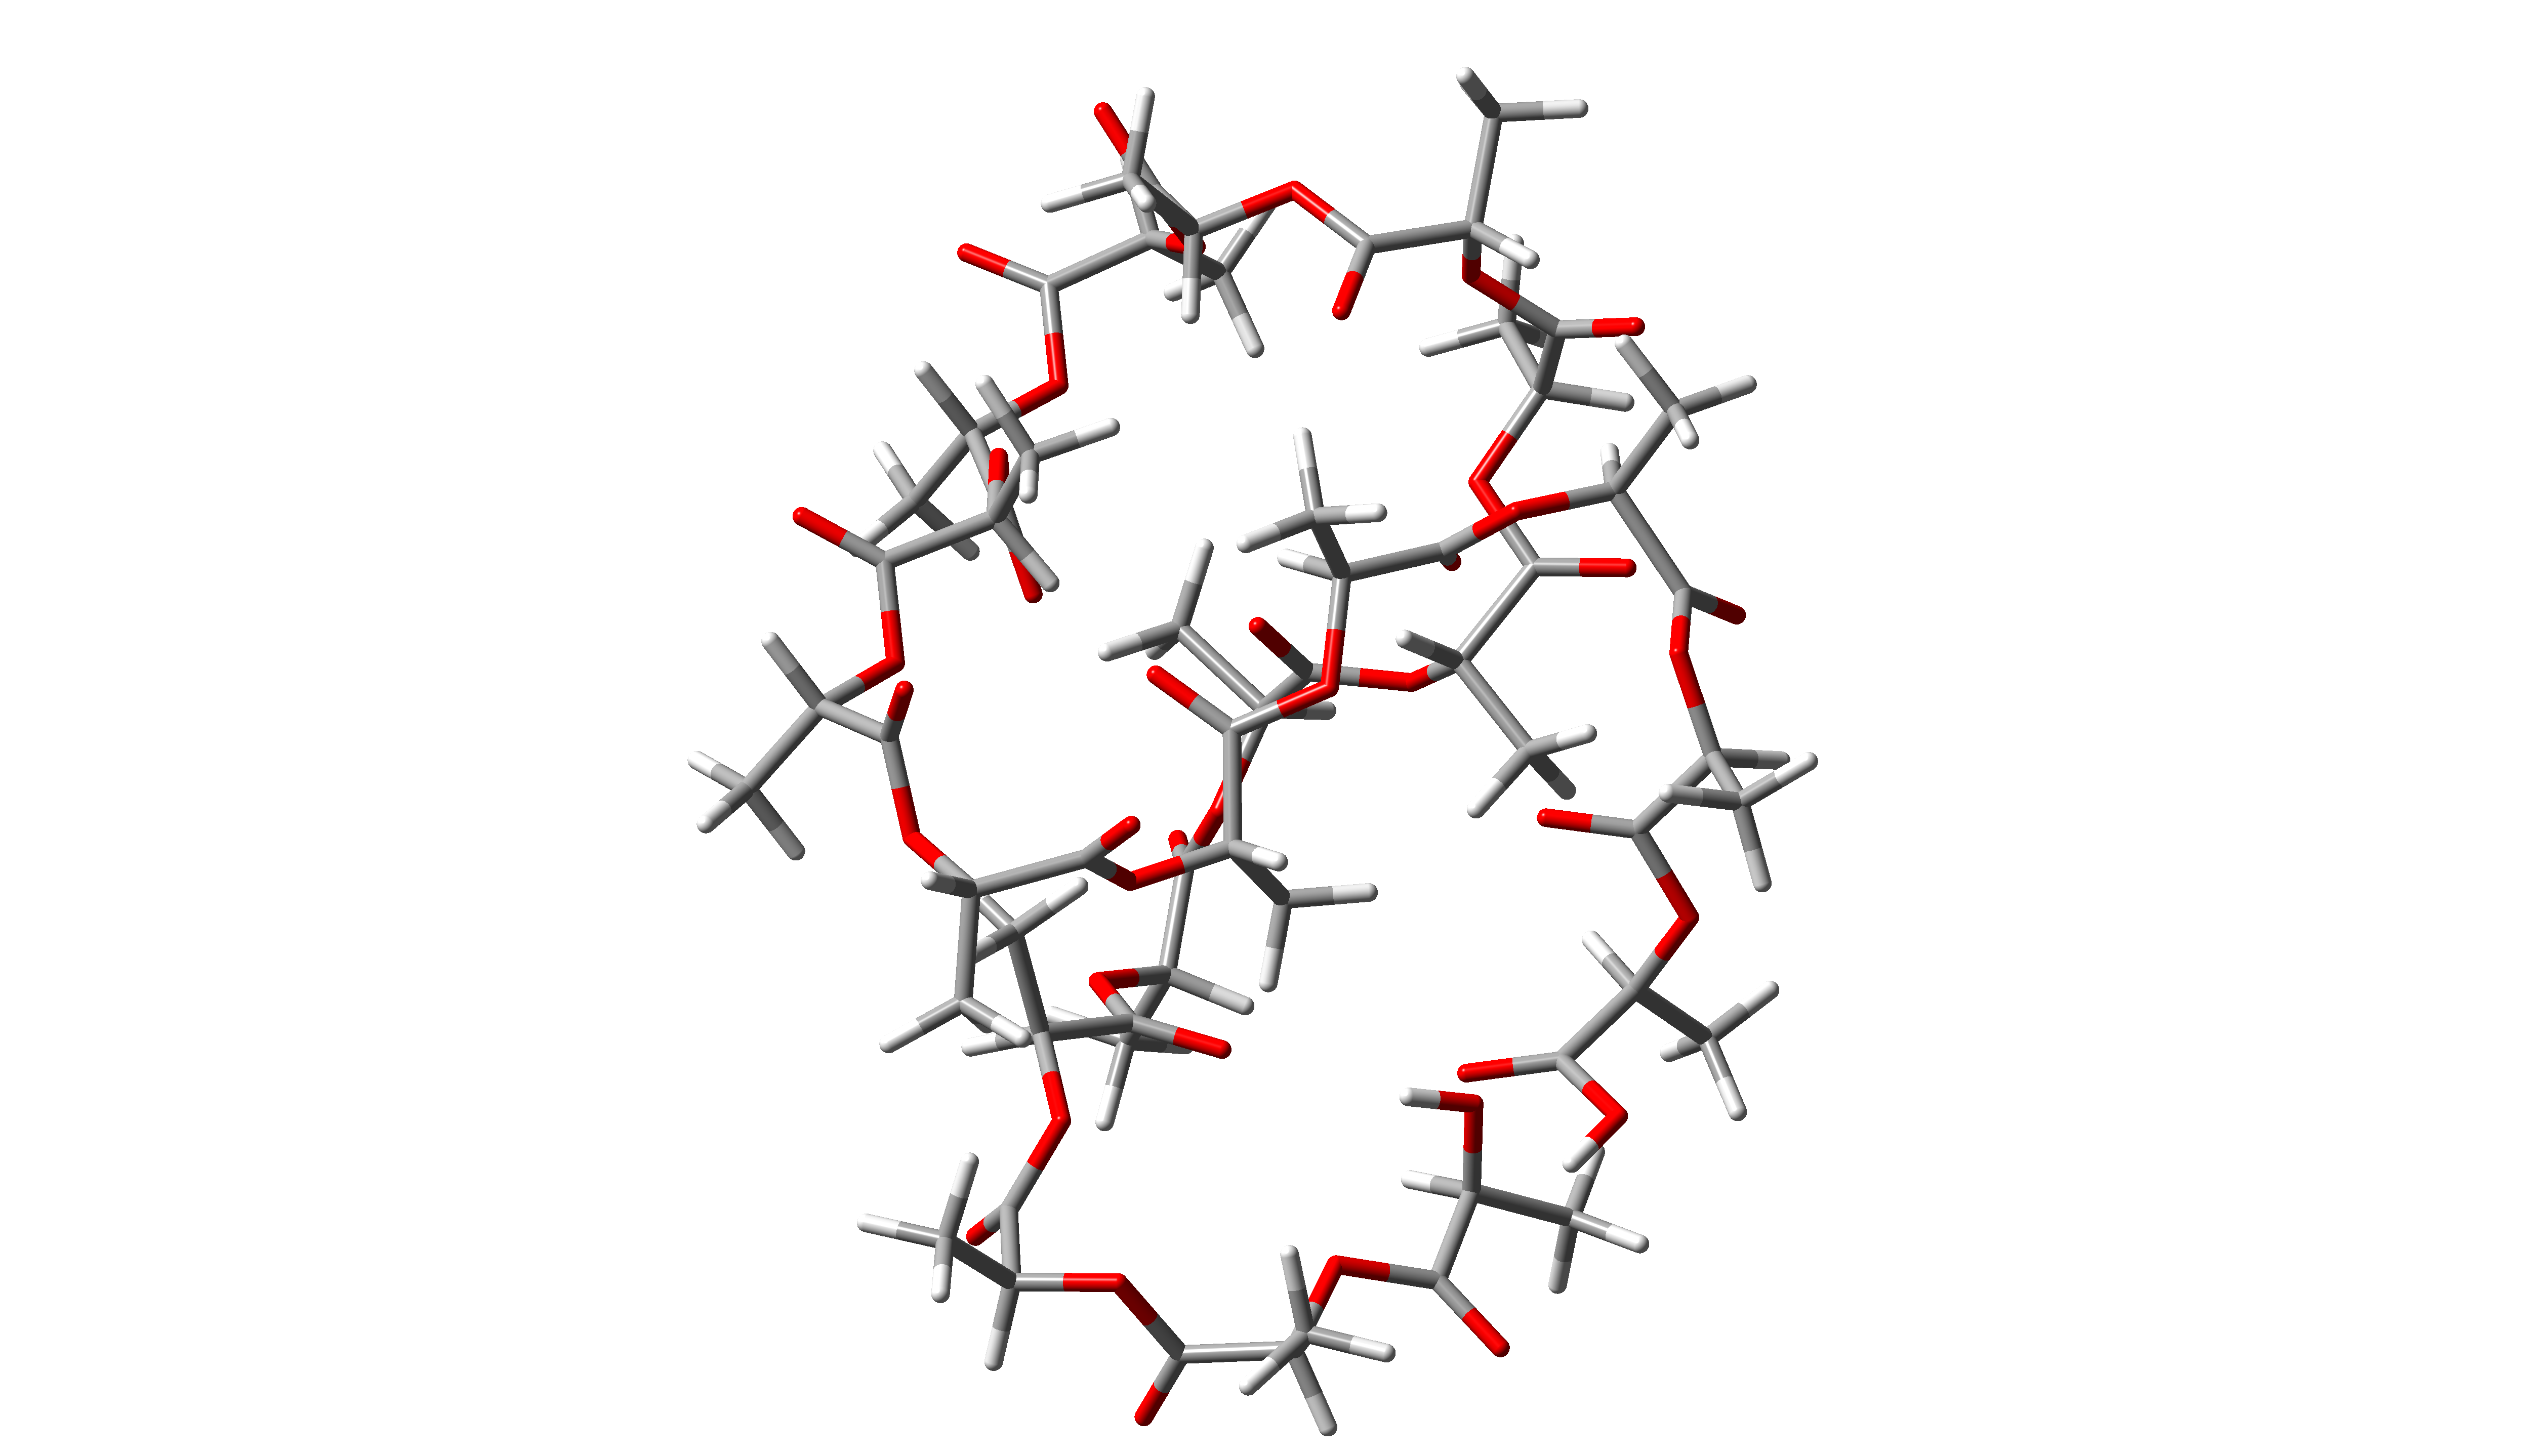
\includegraphics[width=0.9\linewidth]{img/pla_10g_tube.png} 
	\end{subfigure}
	\begin{subfigure}{0.5\textwidth}
		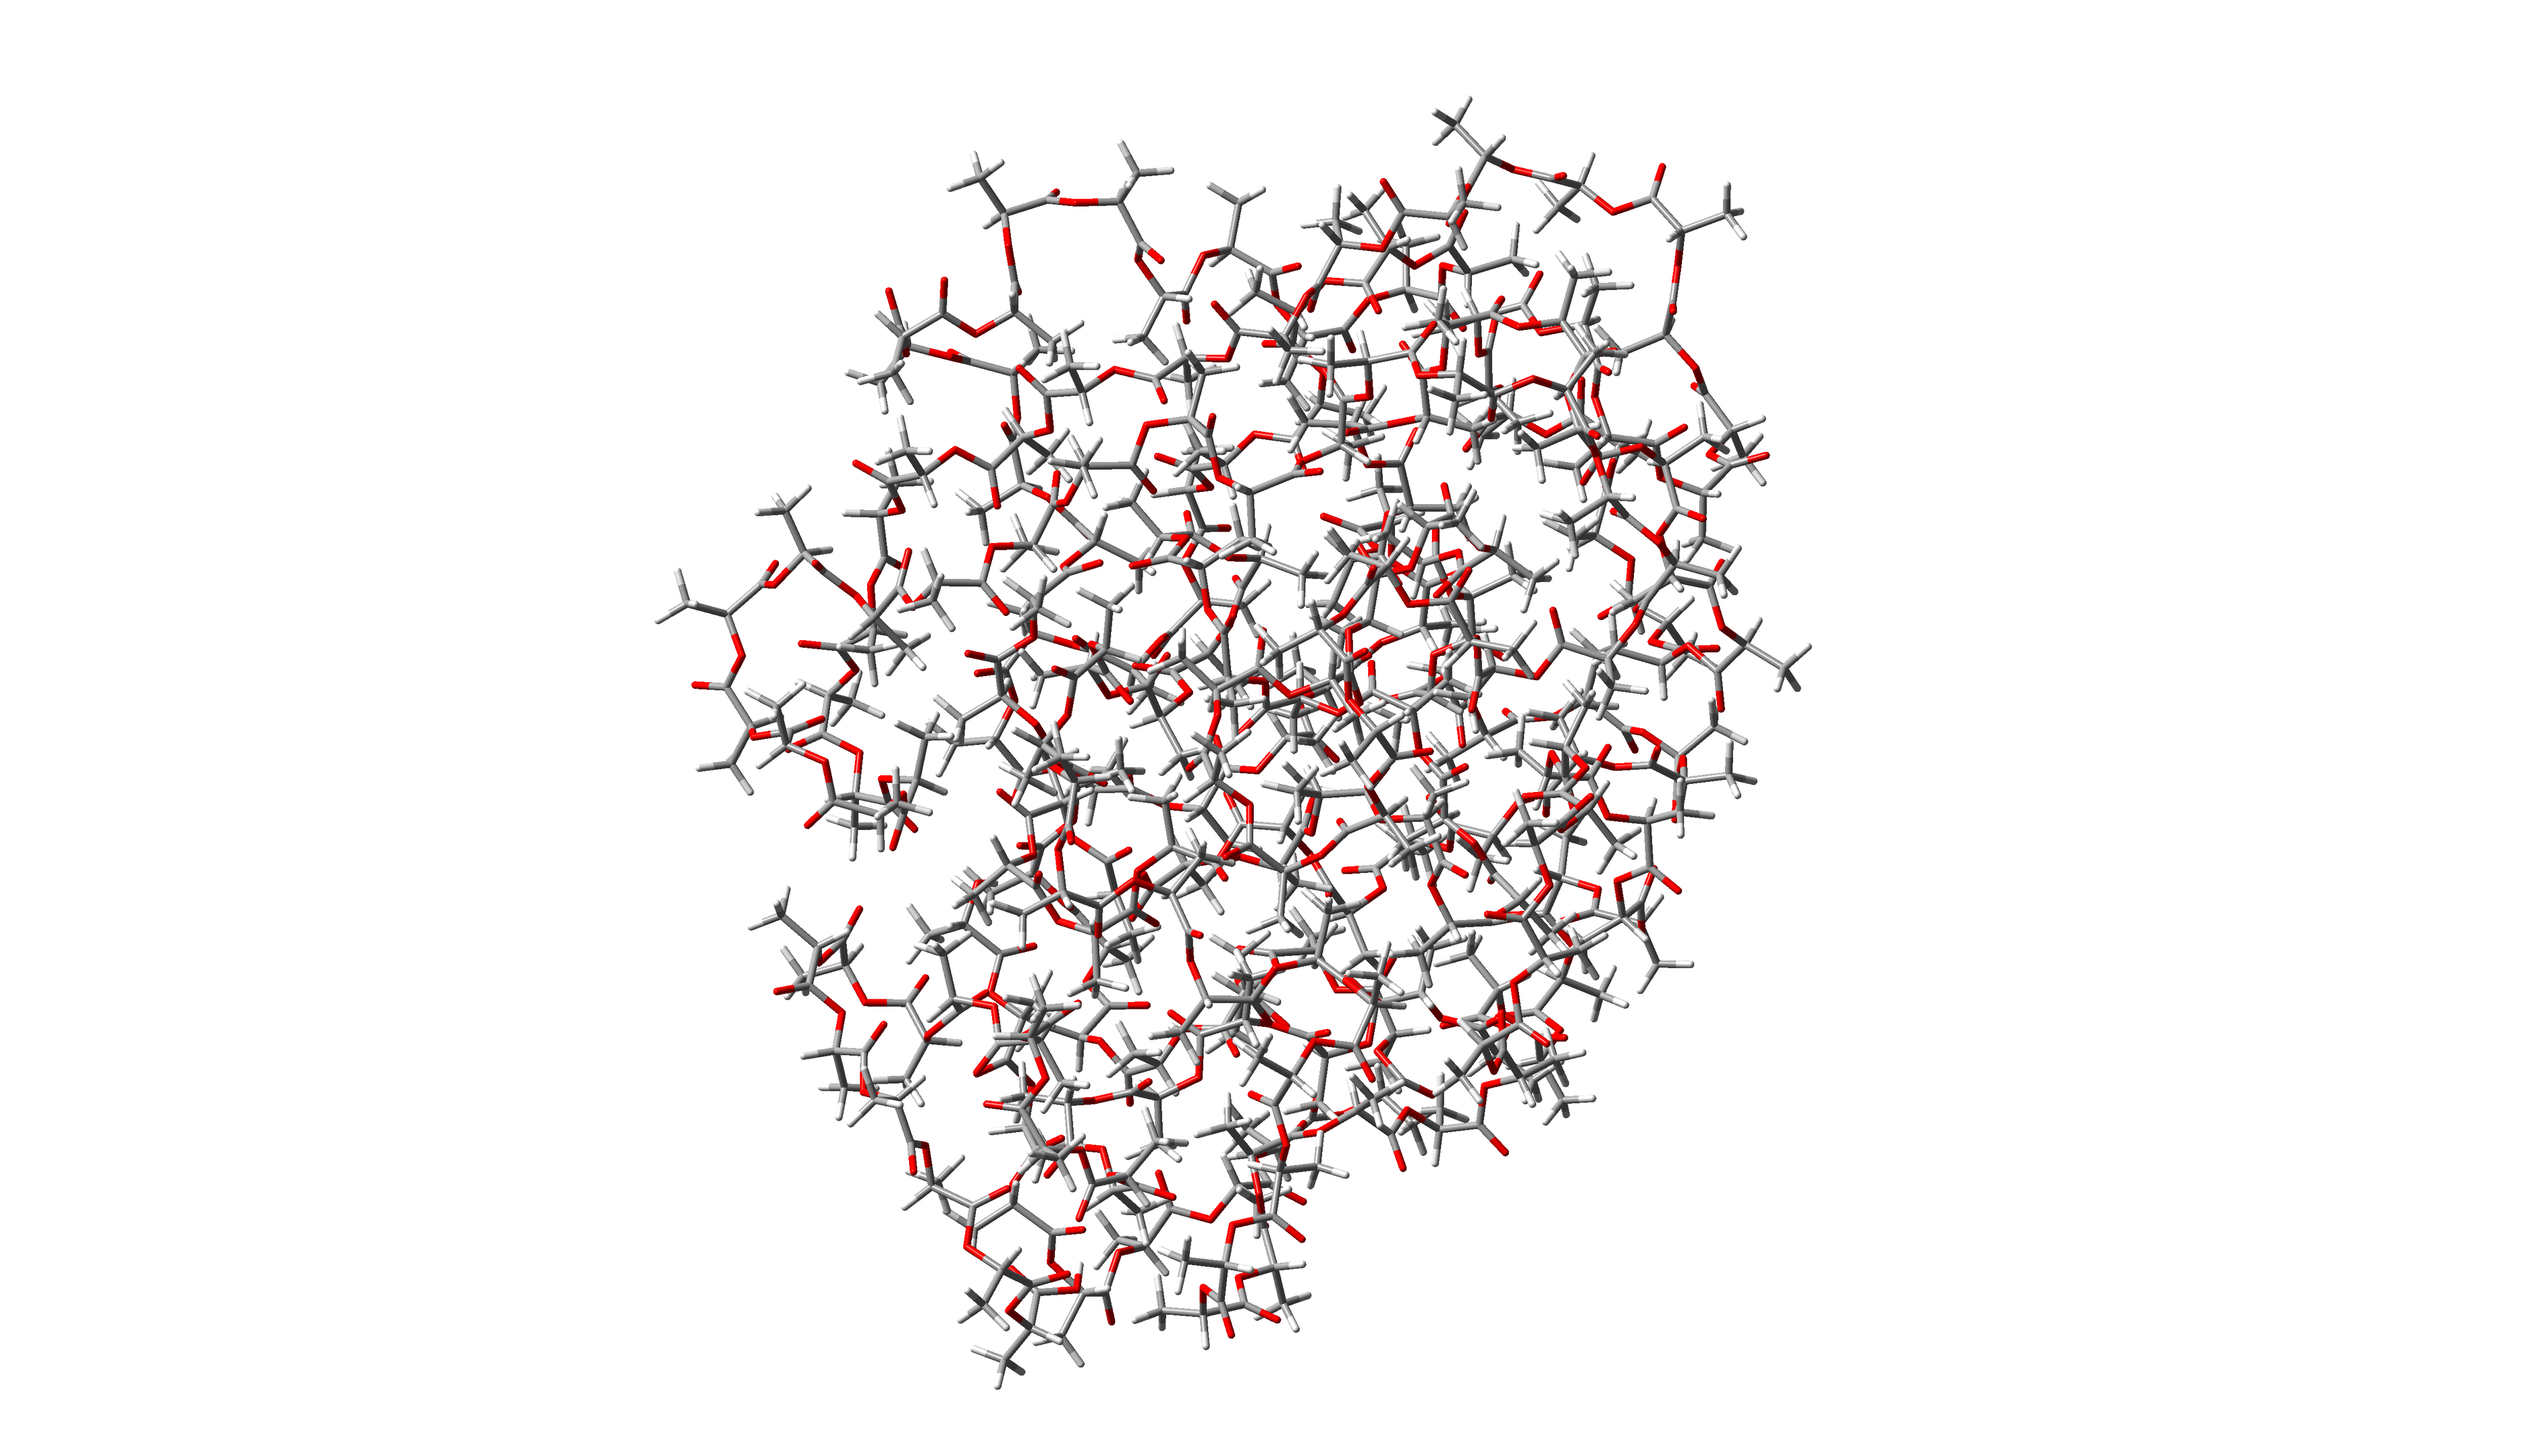
\includegraphics[width=0.9\linewidth]{img/pla_100g_tube.png} 
	\end{subfigure}   	
	\caption{Globular PLA polymer chain, 20 and 200 units}
	\label{fig:sbalene}
\end{figure}

To see the effects of initial conformations, molecular weight and thermal history of the polymer on bulk densities following simulations were performed. The design of the simulation boxes is in Table \ref{tab:pla_chains}. The simulations were first performed at the temperature of 500 K (run 1), then the box was heated up to 1000 K followed by re-cooling and simulating at a temperature of 500 K (run 2). All subsequent simulations were observing the system for 10~ns with a step 1 fs at 1 bar. From these simulations, the densities and the root mean square distance of the polymer chain termini with their standard deviations were evaluated.

\begin{table}[h]
	\centering
	\caption{Design of the neat PLA simulation boxes}
	\label{tab:pla_chains}
	\begin{tabular}{ccccc}
		\toprule
		\textbf{\boldmath$N_{\text{units}}$} & \textbf{\boldmath$n_{\text{chains}}$} & \textbf{\boldmath$N_{\text{atoms}}$} & \textbf{\boldmath$M$, g mol$^{-1}$} & \textbf{\boldmath$d$, \AA} \\
		\midrule
		20 & 140 & 25620 & 1459.3 & 67.9 \\
		40 & 70 & 25410 & 2900.5 & 67.7 \\
		60 & 40 & 24978 & 4341.8 & 64.3 \\
		80 & 35 & 25305 & 5783.1 & 67.7 \\
		100 & 28 & 25284 & 7224.3 & 67.7 \\
		120 & 23 & 24909 & 8665.6 & 67.3 \\
		140 & 20 & 25260 & 10106.8 & 67.6 \\
		160 & 17 & 24531 & 11548.1 & 67.0 \\
		180 & 15 & 24345 & 12989.4 & 66.8 \\
		200 & 14 & 25242 & 14430.6 & 67.6 \\
		\bottomrule
	\end{tabular}
\end{table}

The following graphical representation of the results (Figure \ref{fig:pla_hustoty}) shows a trend of an increasing density depending on the length of the chain (molecular weight), which is independent of the initial conformation of the molecule. There is also visible that densities for longer chains converge to constant value. From this finding, we can consider a system above $M_\mathrm{w}$~=~9~000~$\mathrm{g \ mol^{-1}}$ as sufficiently polymeric.

\begin{figure}[htb!]
	\begin{subfigure}{0.5\textwidth}
		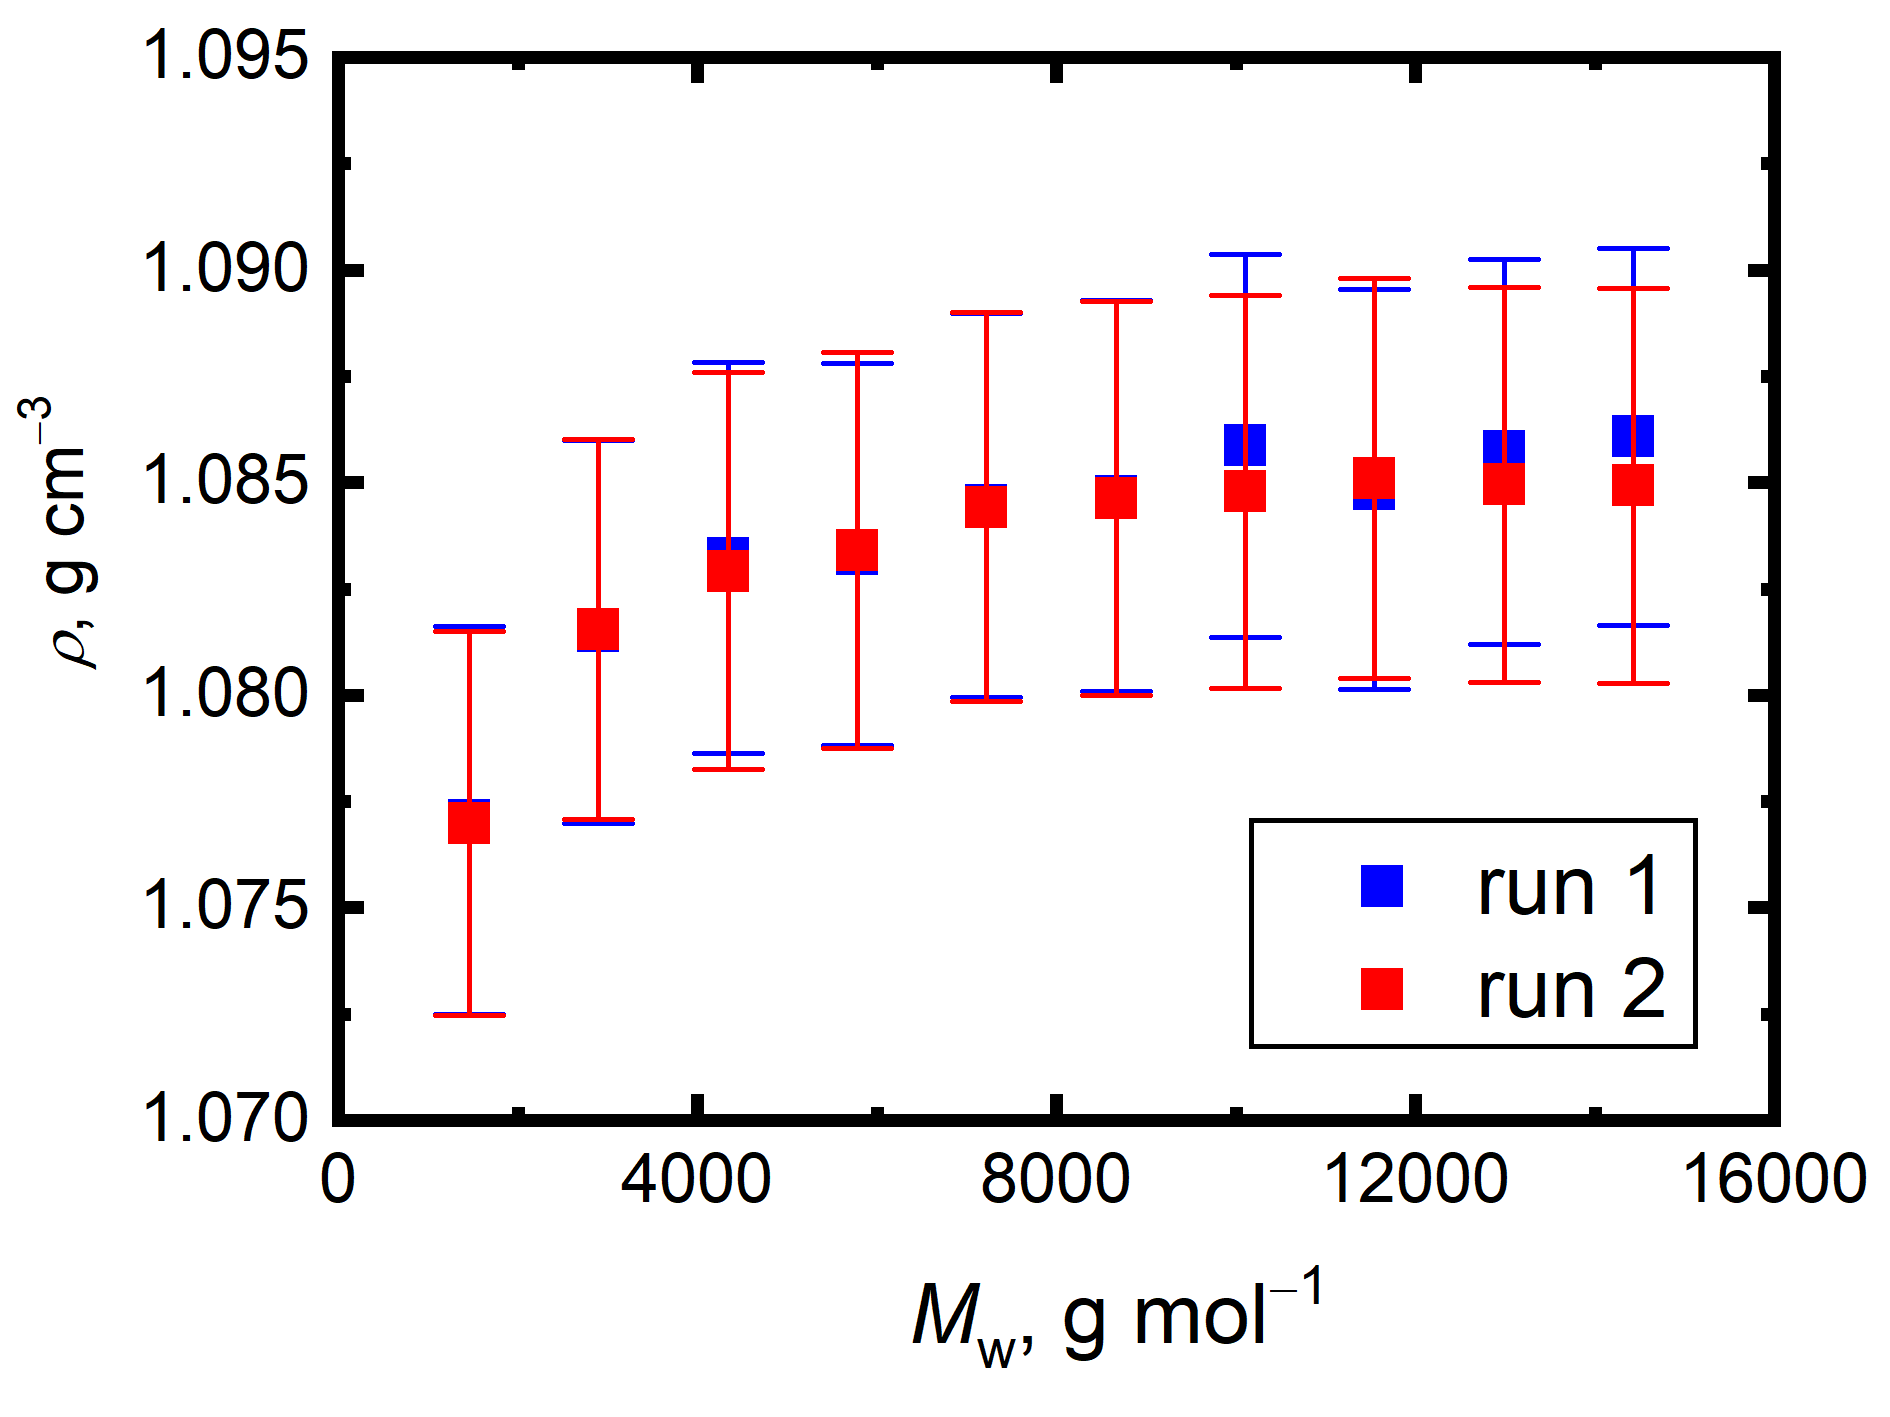
\includegraphics[width=1.0\linewidth]{img/pla_linear_density.png} 
		\caption{from initial fibrilar conformation}
		\vspace{-0.2cm}
	\end{subfigure}
	\begin{subfigure}{0.5\textwidth}
		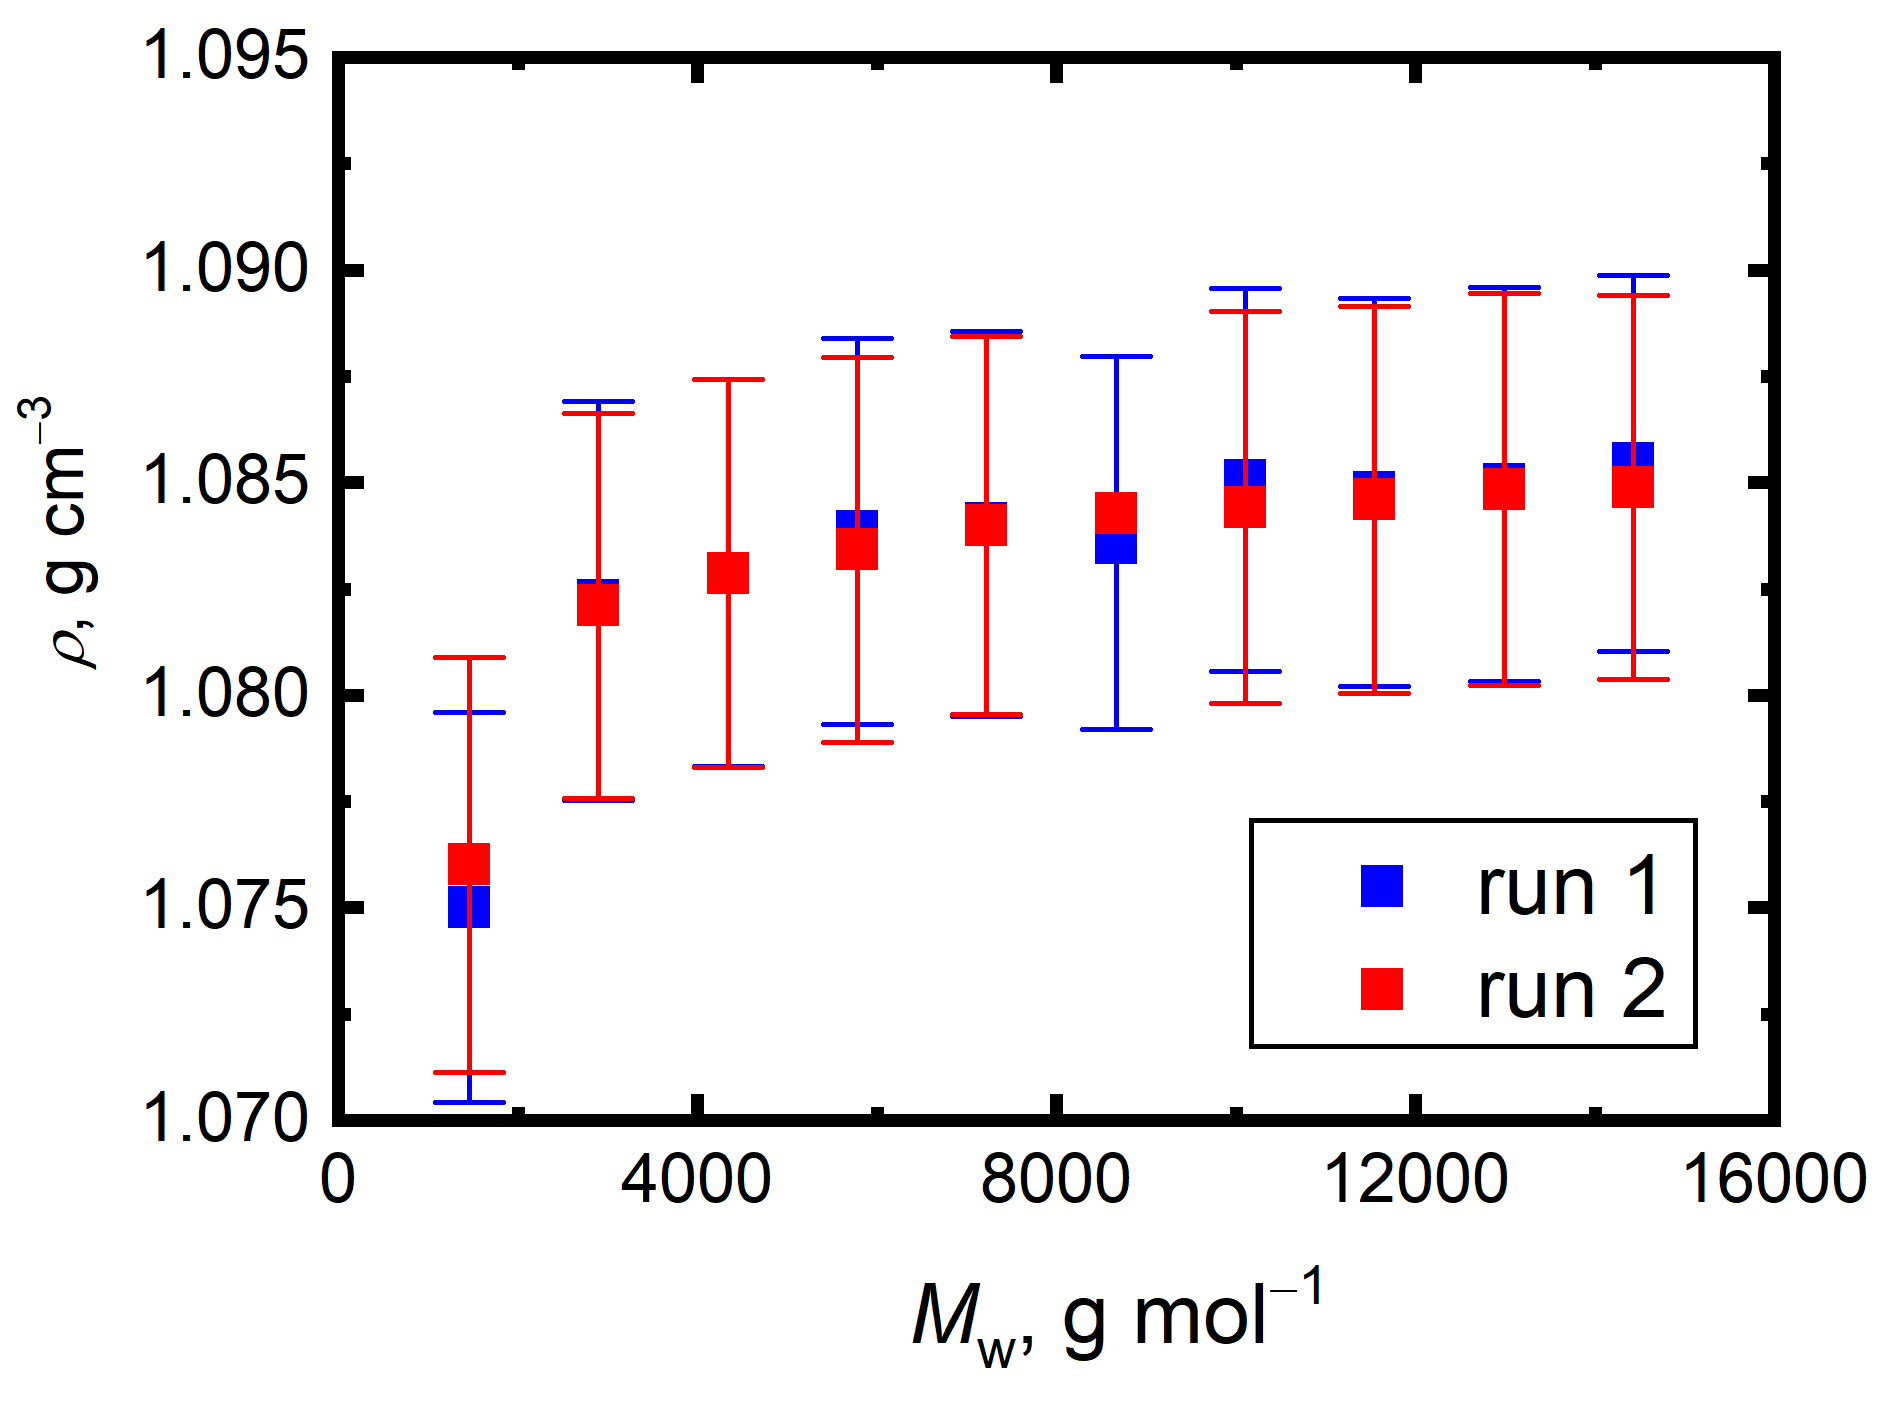
\includegraphics[width=1.0\linewidth]{img/pla_glob_density.png}
		\caption{from initial globular conformation}
		\vspace{-0.2cm}
	\end{subfigure} 
	\caption{Average densities with their standard deviations for PLA polymer chains at 500 K and 1 bar as a function of chain length before (run 1) heating and (run 2) after cooling.}
	\label{fig:pla_hustoty}
	\vspace{-0.2cm}
\end{figure}

From the density data, any impact of the conformation memory cannot be assessed, since the bulk density is too a crude point of view on the polymer structure. That is the reason why the distances of the polymer chain termini that are displayed in the Figure \ref{fig:pla_konce} were calculated. The simulated time of 10 ns at the elevated temperature 1000 K was not enough to completely erase the polymer conformational memory, there is a noticeable deviation of the data sets representing the initial fibrilar and globular conformations.

\begin{figure}[htb!]
	\begin{subfigure}{0.5\textwidth}
		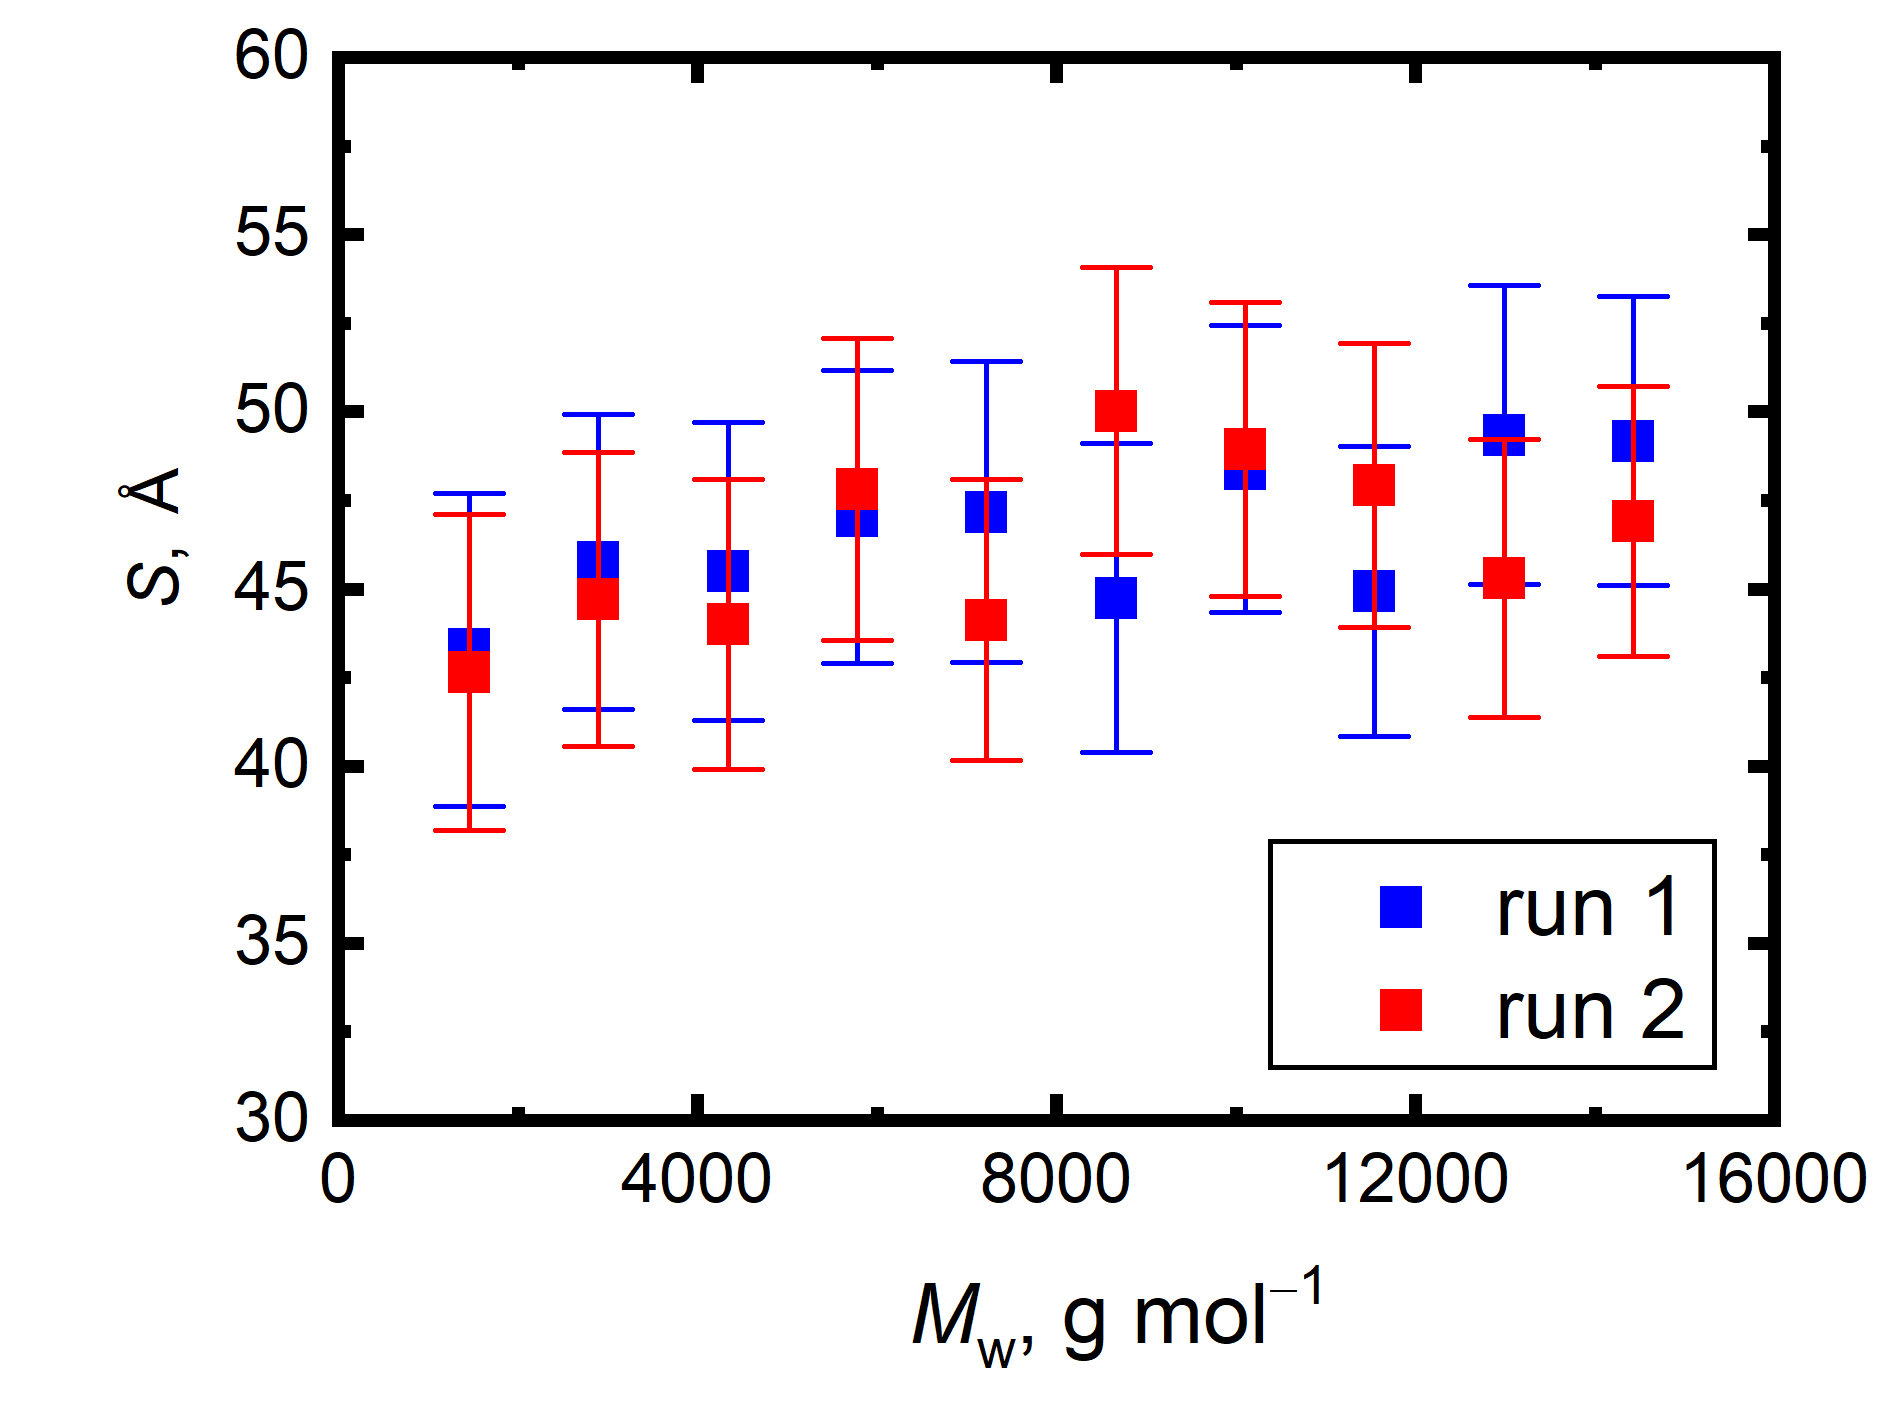
\includegraphics[width=1.0\linewidth]{img/pla_linear_konce.png} 
		\caption{from initial fibrilar conformation}
		\vspace{-0.2cm}
		\label{fig:subim1}
	\end{subfigure}
	\begin{subfigure}{0.5\textwidth}
		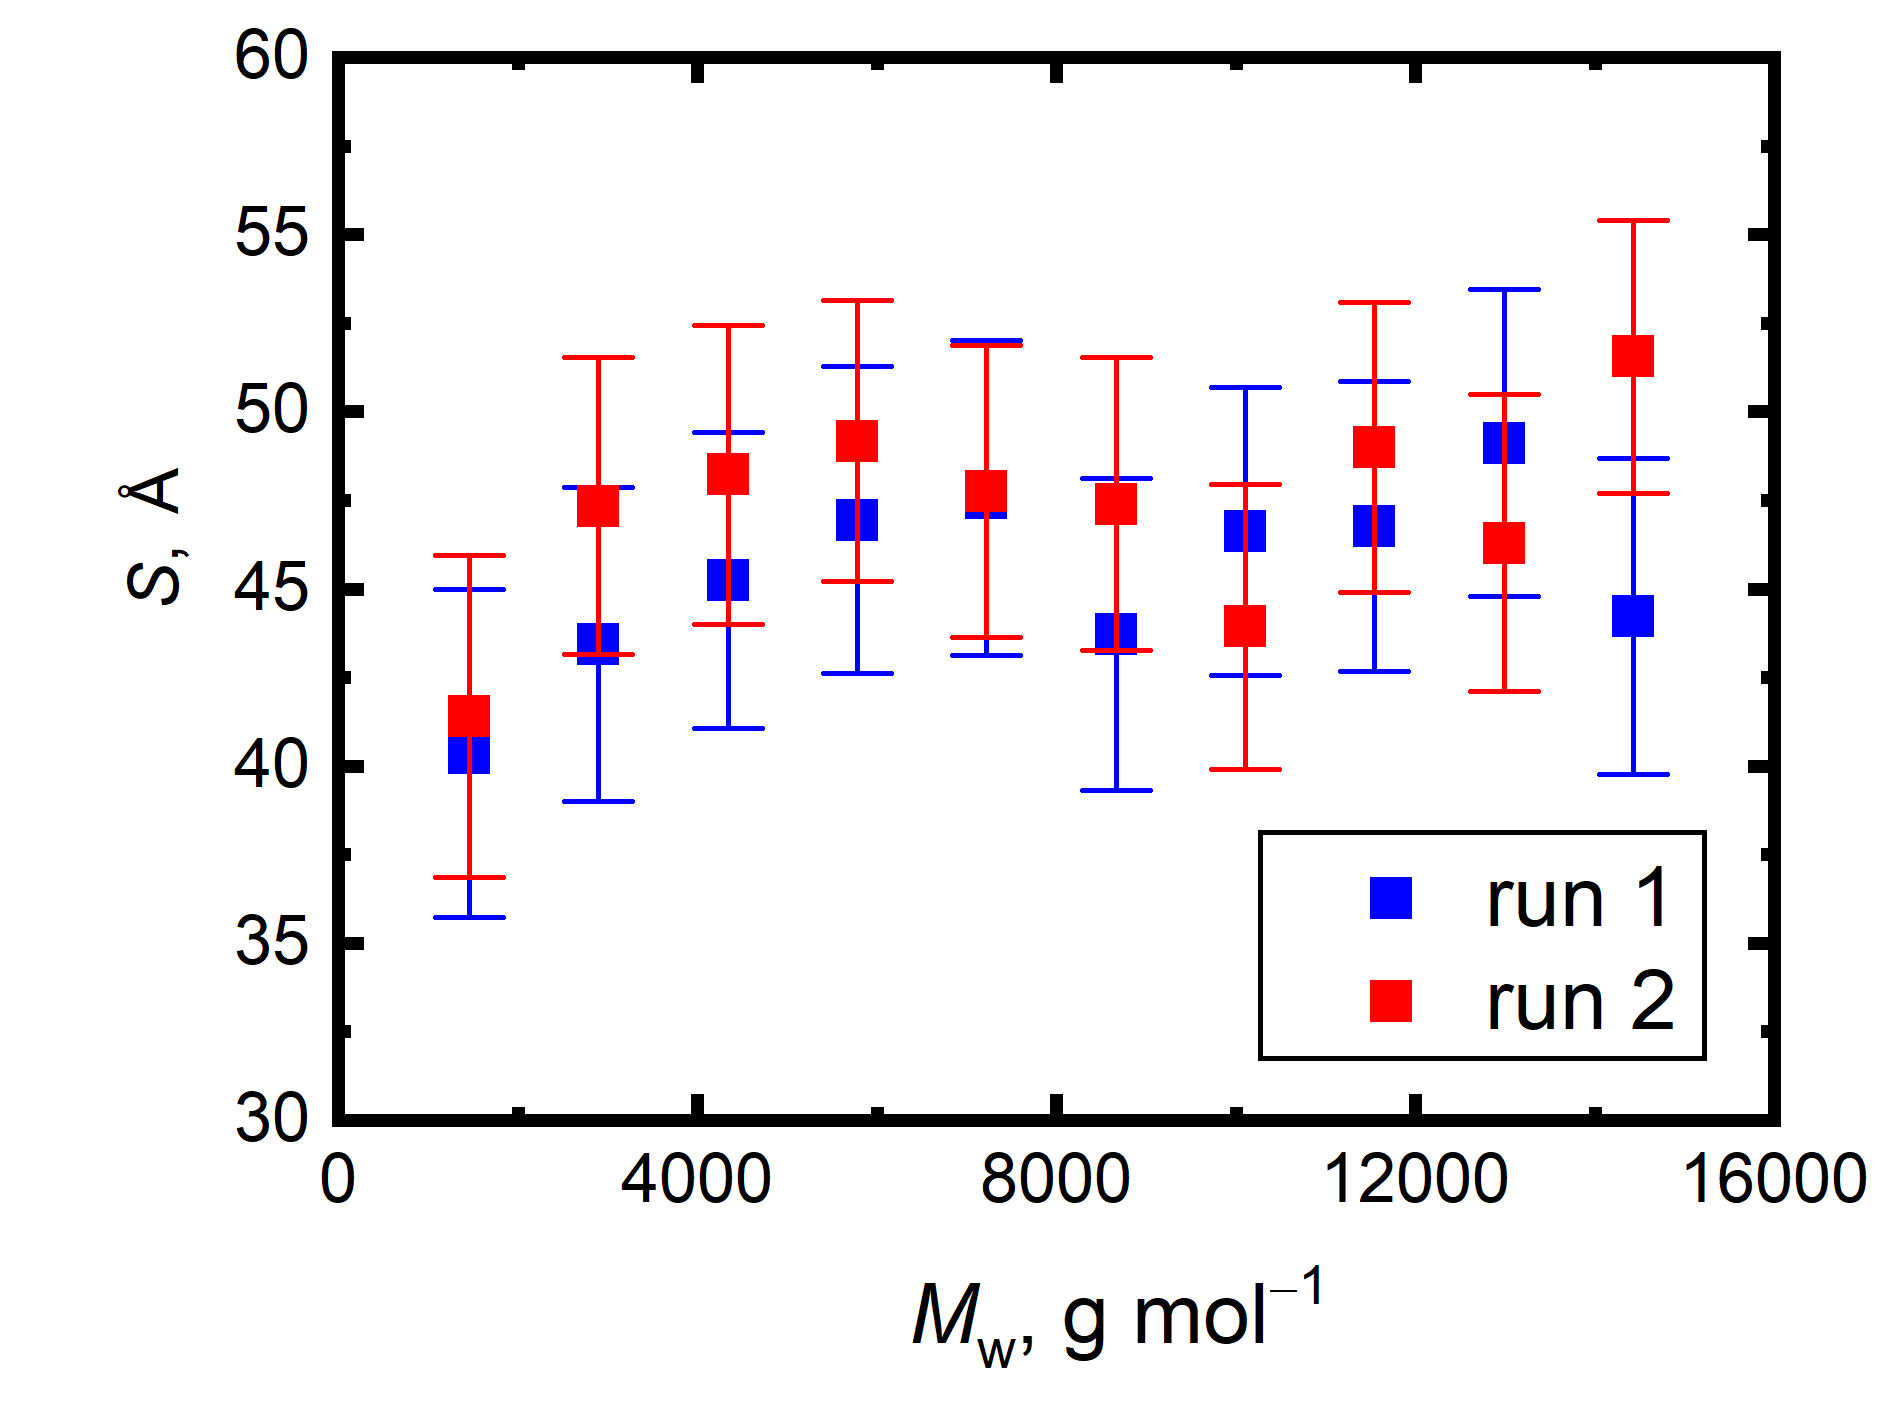
\includegraphics[width=1.0\linewidth]{img/pla_glob_konce.png}
		\caption{from initial globular conformation}
		\vspace{-0.2cm}
		\label{fig:subim2}
	\end{subfigure}
	\caption{Distances of the polymer chain termini with their standard deviations  for PLA polymer chains as a function of chain length before (run 1) heating and (run 2) after recooling.}
	\label{fig:pla_konce}
\end{figure}      

The dynamics of the polymer is slow due to complex entanglement of individual chains even at elevated temperatures, for a complete loss of memory it would be necessary to simulate the system for a longer period of time, especially for longer chains.

To investigate the effect of the box size on the molecular simulations, the simulations with box containing 5-50 polymer chains inside, each having a molar mass 12 989 $\mathrm{g \ mol^{-1}}$ were performed. The simulations were performed with a 3-block initial equilibration at 1000 K and 1 bar and subsequently cooled to 500 K and simulated for 10 ns. Mean densities obtained from these simulations are shown in the Figure \ref{fig:box} on the left. The simulation results prove that the initial size of the box has no significant effect on resulting average density. However, there is a visible effect of a lower uncertainty of standard deviations of densities for larger boxes. To have a better insight what is going on the structural level, we also analyzed the root-mean-squared end-to-end distance of the polymer chain termini shown in Figure \ref{fig:box_konce} on the right. From the obtained data there is visible growing trend in end-to-end distances. That means that the small boxes do not represent correctly the distribution of the end-to-end distances in the polymer. We can say, that the value converge for box containing more than 40 polymer chains. As a conclusion, when we are focused on macroscopic values such as density we can use smaller number of chains in the simulation boxes in order to save the computational resources. However, when dealing with structural properties we should be careful and set the number of chains in a simulation box more carefully.

\begin{figure}[htb!]
	\begin{subfigure}{0.5\textwidth}
		\centering
		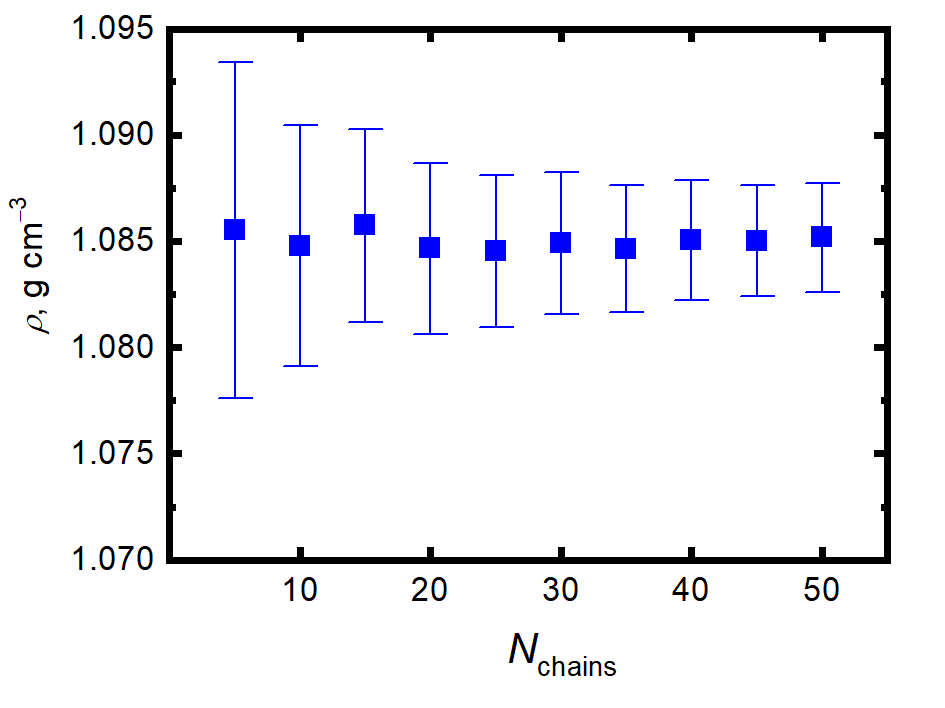
\includegraphics[width=1\linewidth]{img/box_density_5_50.png}
		\caption{}
		\label{fig:box}
	\end{subfigure}
	\begin{subfigure}{0.5\textwidth}
		\centering
		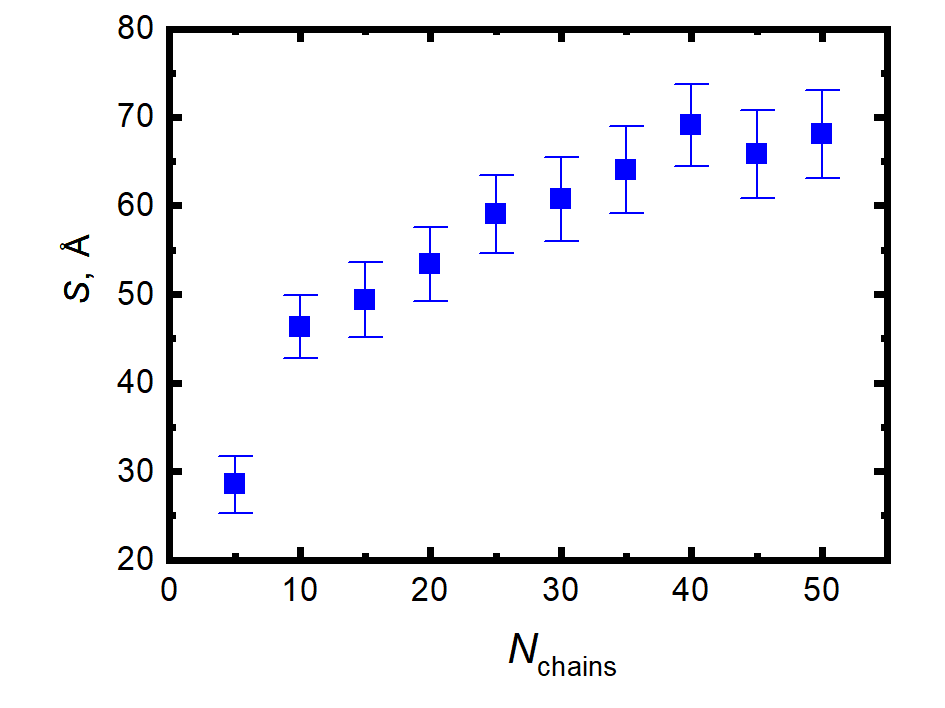
\includegraphics[width=1\linewidth]{img/konce_5_50.png}
		\caption{}
		\label{fig:box_konce}
	\end{subfigure}   	
	\caption{(a) dependence of density on number of chains containing 90 dimer units in the box on the left and (b) density of PLA at 500 K and 1 bar extracted from MD simulations depending on the polydispersity coefficients on the right.}
	\vspace{-0.2cm}
\end{figure}

To validate the calculated densities, the corresponding experimental data was obtained from literature. The comparison for two temperatures (300 and 500~K) in following Table \ref{tab:PLA_dens} was taken from \cite{klajmon_glass_2023}, where the methodology is also described in more details.

\begin{table}[htbp]
	\centering
	\caption{Comparison of calculated and experimental PLA denstities taken from \cite{klajmon_glass_2023}.}
	\begin{tabular}{ccc}
		\toprule
		$T$, K & $\rho_{\text{exp}}$ & $\rho_{\text{calc}}$ \\
		\midrule
		 300   & $1.373 \pm 0.003$ & $1.193 \pm 0.001$ \\
		 500   & $1.181 \pm 0.003$ & $1.086 \pm 0.001$ \\
		\bottomrule
	\end{tabular}%
	\label{tab:PLA_dens}%
\end{table}%

\subsubsection{Polydispersity effect}
Under real conditions, it is hardly possible to experimentally prepare a monodisperse polymer containing only one selected chain length. For this reason, we simulated several polydisperse systems, each exhibiting a different distribution of molar masses of individual molecular chains, containing a total number of 50 chains. The lengths come from interval 8-244 units. Polydispersity index PDI~=~1 corresponds to 50 chains of length 124 units, the other values were calculated using the equation \ref{eq:PDI}. We than build the other systems using the Gaussian distribution with mean value of 124 units. By this procedure we were able to obtain the PDI equal to 1.3. For PDI 1.4 and 1.5 we had to adapt the number of very short and long polymers randomly to get the desired PDI. Designed compositions of systems based on PDI values are displayed in the Figure \ref{fig:polydisperzita_vyskyt}. The density was again evaluated from the simulations, in this case as a function of the PDI.

\begin{equation}
	\text{PDI} = \frac{\sum_{i} N_{i} \cdot \sum_{i} N_{i} M_{i}^2}{\left(\sum_{i} N_{i} M_{i}\right)^2}
	\label{eq:PDI}
\end{equation}


\begin{figure}[htb]
	\centering
	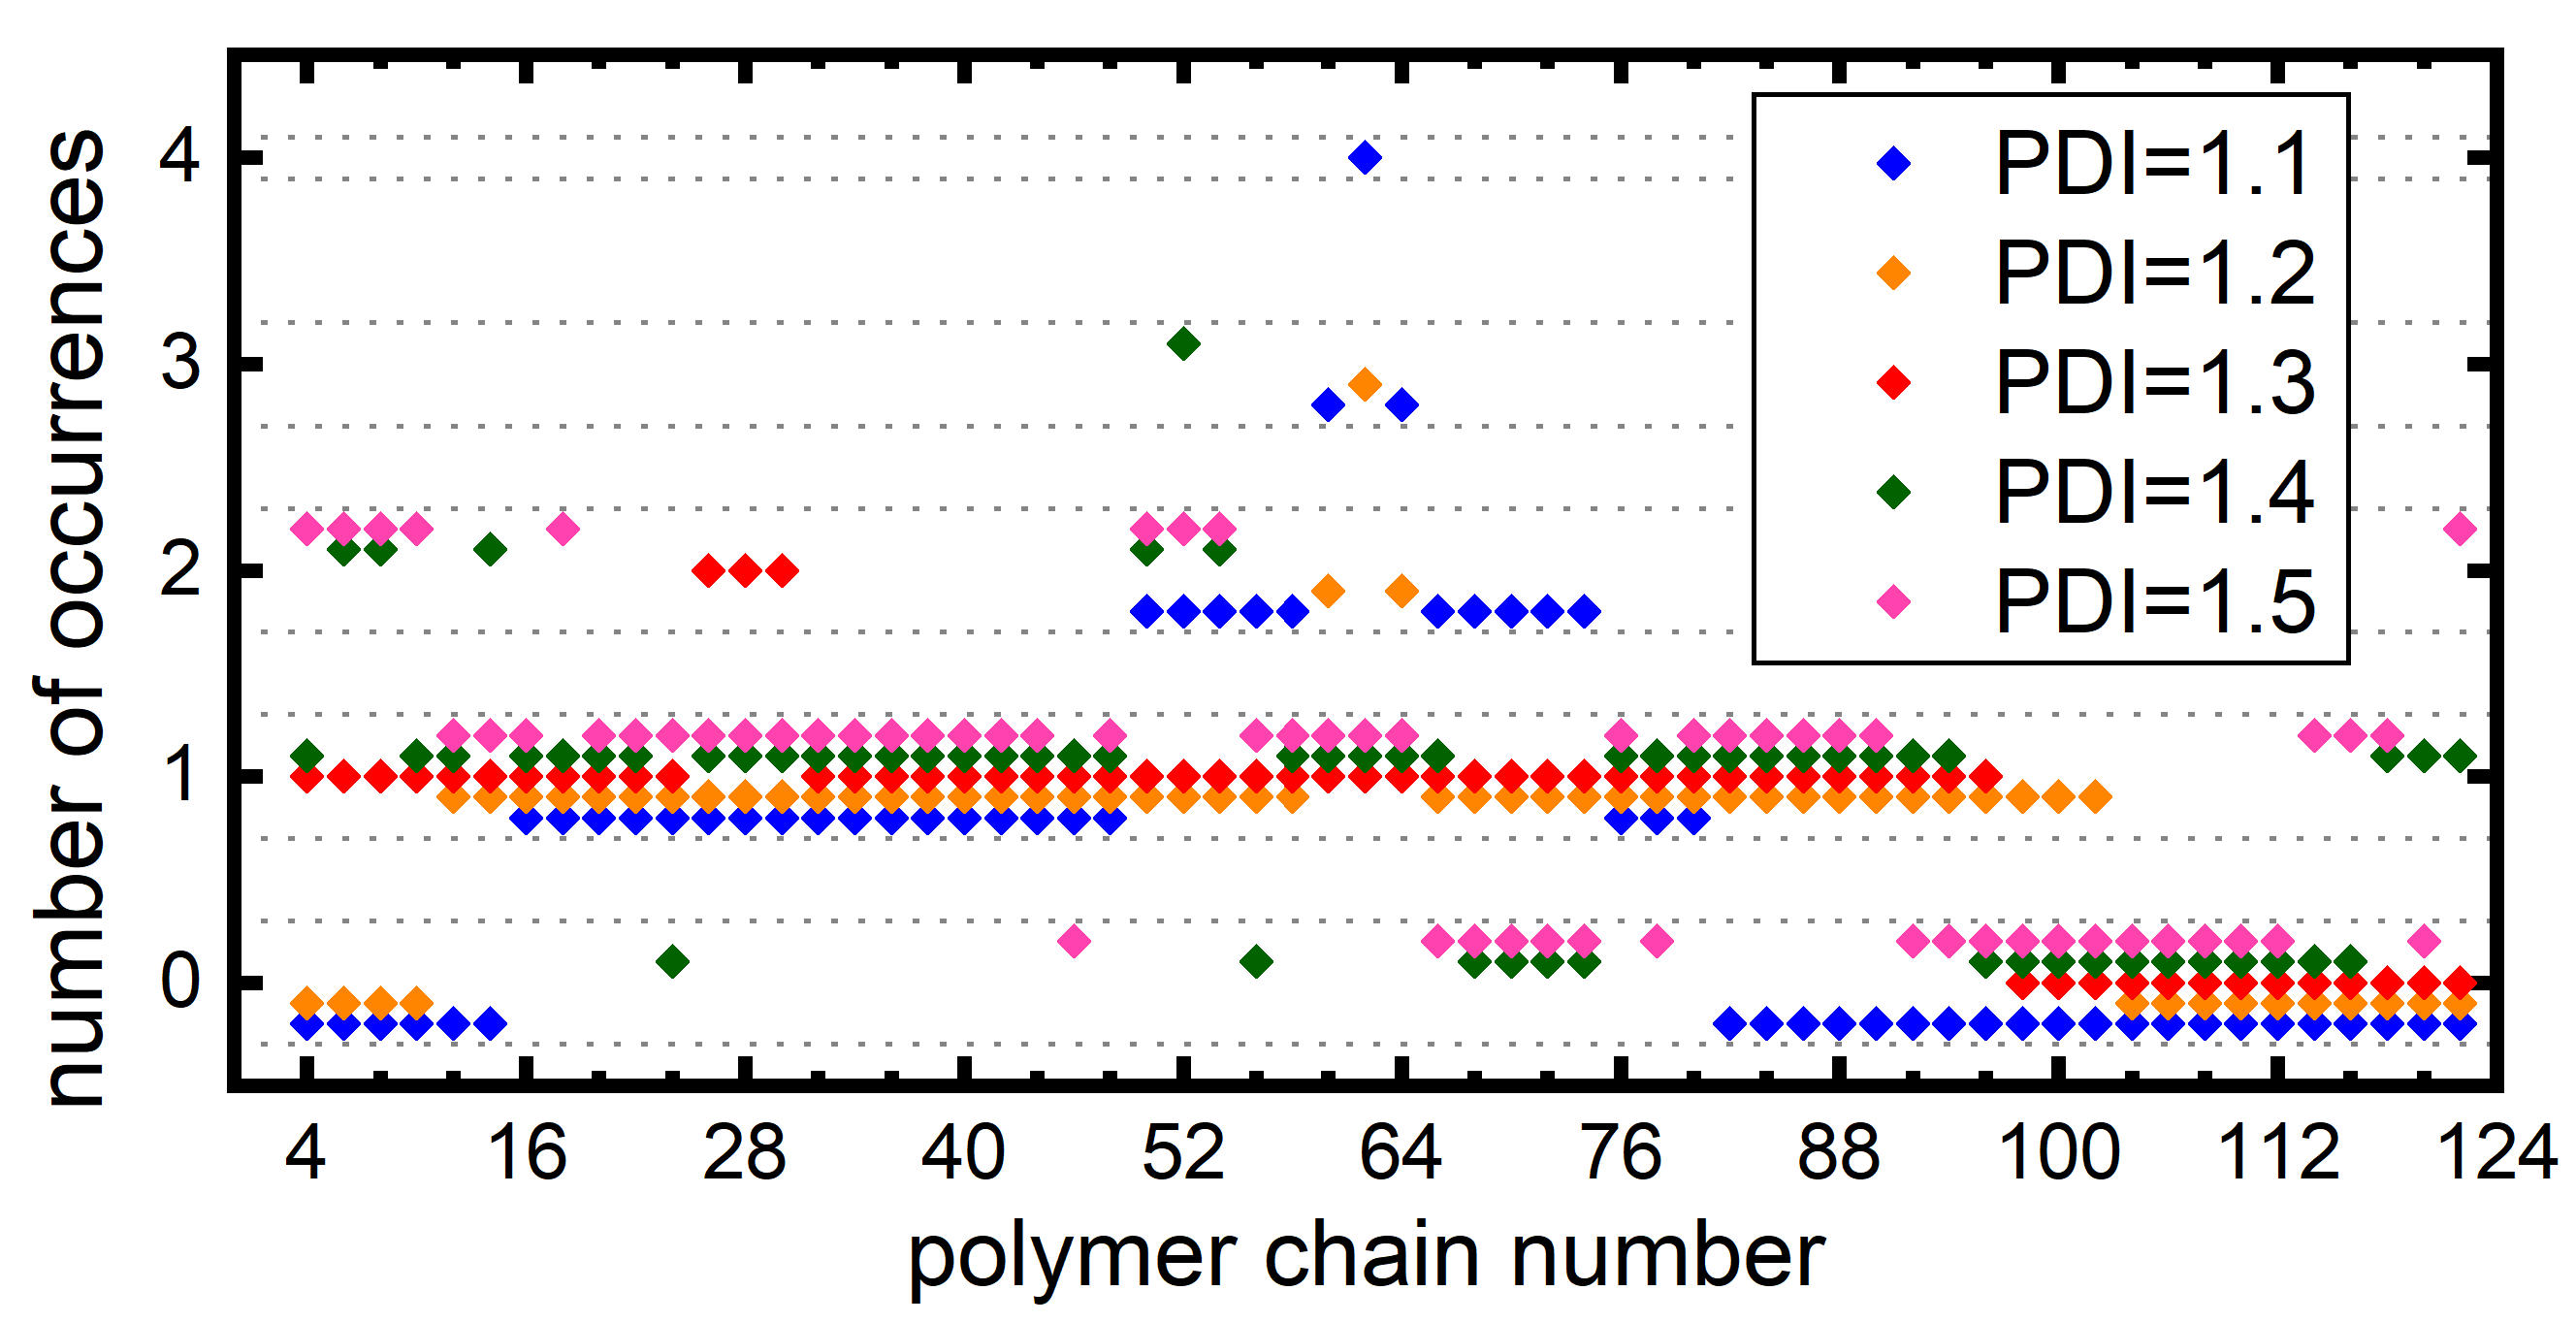
\includegraphics[width=1\hsize]{img/polydispersity_occurrences.png}
	\caption{Number of occurrences of chains of a given length in the polydisperse systems with corresponding PDI.}
	\label{fig:polydisperzita_vyskyt}
\end{figure}       

Calculated densities depending on the PDIs are in the Figure \ref{fig:polydisperzita}. There is not a massive difference among the densities obtained for different values of the polydispersity index, for the subsequent simulations we will use monodisperse systems as it will not introduce big errors. 

\begin{figure}[htb]
	\centering
	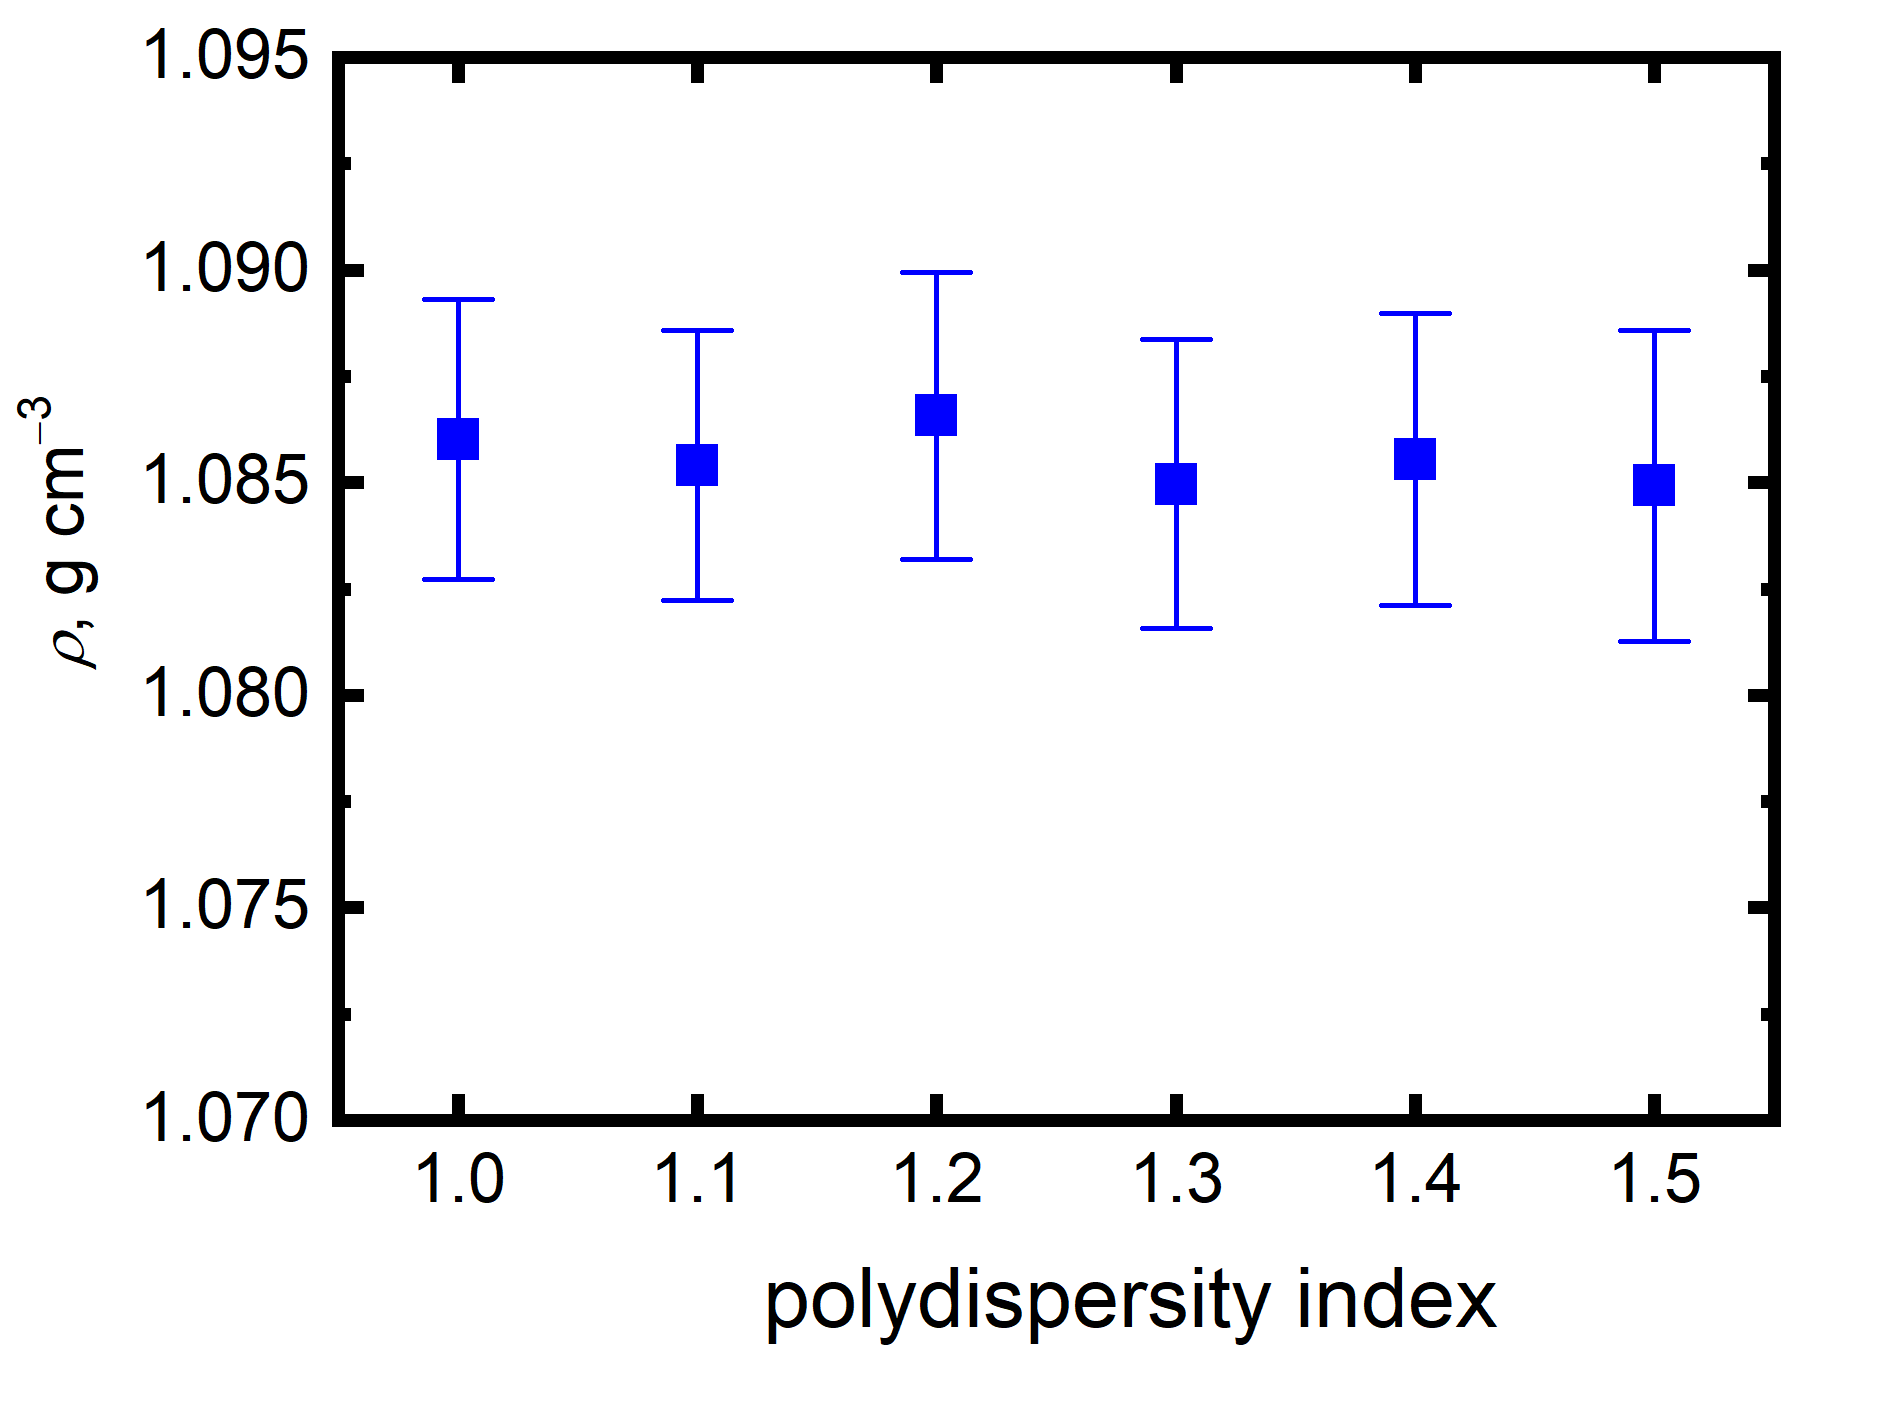
\includegraphics[width=0.5\hsize]{img/polydisperzita.png}
	\caption{Density of PLA at 500 K and 1 bar extracted from MD simulations depending on the polydispersity coefficients.}
	\label{fig:polydisperzita}
\end{figure}       

\subsubsection{Glass transition modeling}
To obtain the glass transition temperature of PLA ($T_\mathrm{g}$), we started by simulating ten different polymer chain lengths for a set of temperatures in a range 140-485 K with a step of 15 K. For the system equilibration, each polymer chain simulation runs for 1 ns with a step of 1 fs. After the equilibration, the temperature interval for the following simulations was limited to the range of 200-485 K with a step of 15 K. Then, we run a $NpT$ production simulation with this limited temperature interval for 10 ns with a step of 1 fs from which the equilibrium bulk phase densities were calculated and displayed as a function of temperature. To get the glass transition temperature ($T_\mathrm{g}$) for PLA from that function, the trend shift method was used \cite{klajmon_does_2022}. 

The trend shift method is illustrated for one length of the polymer chain in the Figure \ref{fig:glass}. When we plot the bulk phase densities as a function of temperature, there is a visible trend shift which has the meaning of the transition between the glassy state and the rubbery state. The point of the transition divides the density dataset into two intervals. Coordinates of the breakpoint and one surrounding point from each side were excluded from the further processing and the two resulting intervals were interpolated by a linear function. The $x$-coordinate of the intersection of these two lines determines the glass transition temperature. For this purpose a script in Maple software solving the system of linear equations to get the $T_\mathrm{g}$.

Available experimental $T_\mathrm{g}$ of L-PLA varies in the literature, the value  of $T_\mathrm{g}$ = 333 $\pm$ 4~K \cite{pyda_reversing_2005} was chosen. Our obtained PLA $T_\mathrm{g}$ = 337 $\pm$ 10~K as an arithmetic mean of the values for all polymer chain lengths. The calculated $T_\mathrm{g}$ for each polymer chain are displayed as function of polymer chain weight in the Figure \ref{fig:glass} with their arithmetic mean value drawn as a blue line. The calculated $T_\mathrm{g}$ value is very close to the experimental one. There is no significant trend in $T_\mathrm{g}$ of PLA from the calculated data. 


\begin{figure}[H]
	\begin{subfigure}{0.5\textwidth}
		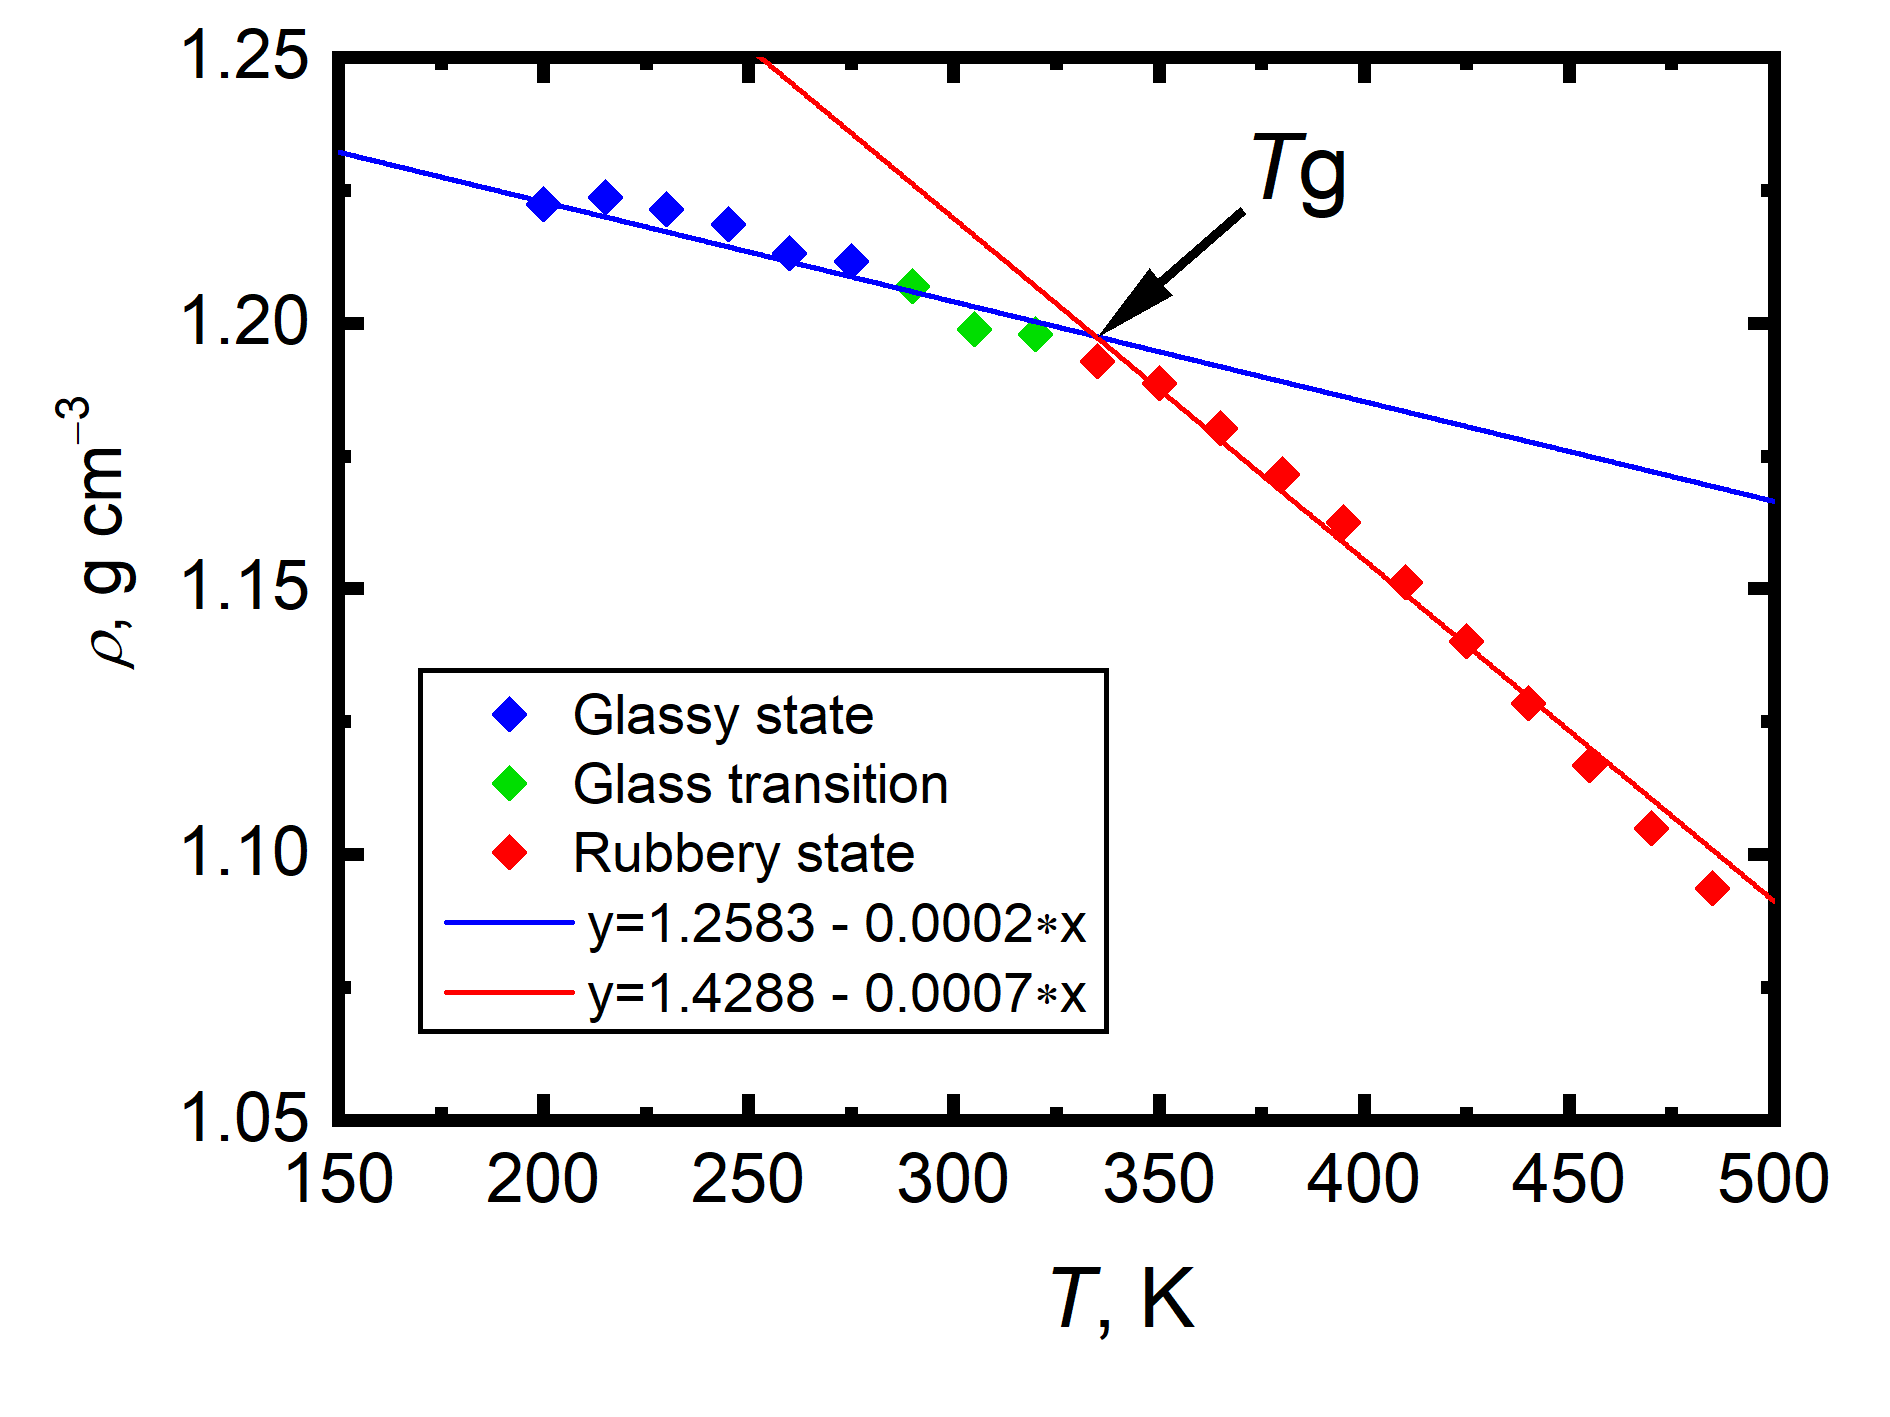
\includegraphics[width=1.0\linewidth]{img/vypocet_tg.png} 
	\end{subfigure}
	\begin{subfigure}{0.5\textwidth}
		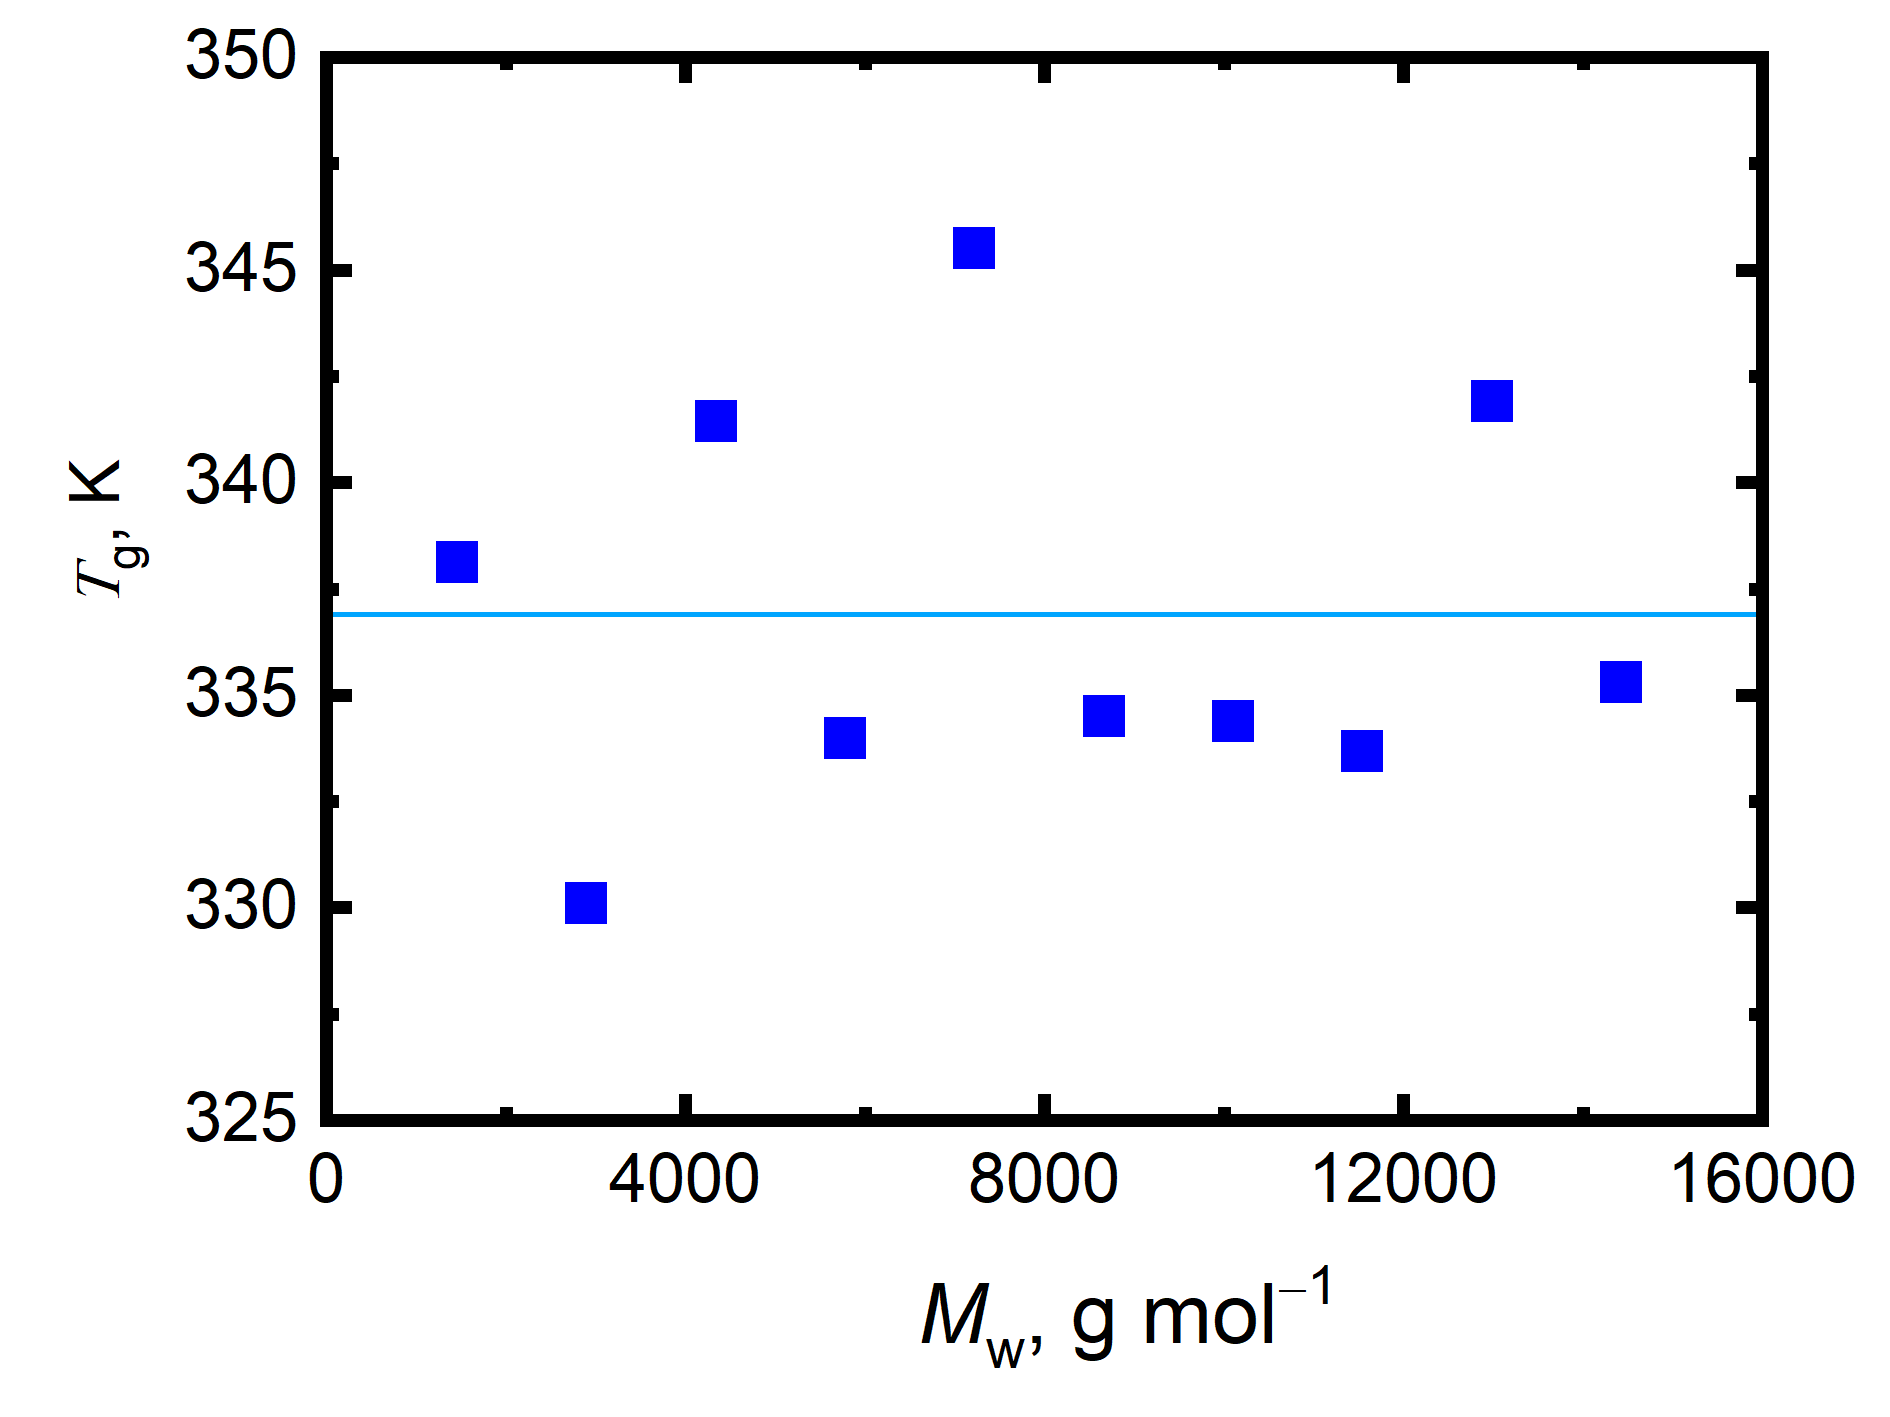
\includegraphics[width=1.0\linewidth]{img/glass_temp.png} 
	\end{subfigure}   	
	\vspace{-1cm}
	\caption{Illustration of the trend shift method for one polymer chain length on the left, and calculated $T_\mathrm{g}$ for all lengths of polymer chains by this method where blue line represents mean value on the right.}
	\label{fig:glass}
\end{figure}

\newpage
\subsection{Simulations of neat API}
The properties of API simulation boxes after equilibration run ($T$=500 K) is presented in Table \ref{tab:API_n}, showing the number of API molecules ($N_{\text{API}}$), the total number of all atoms ($N_{\text{atoms}}$) and size of the cubic box ($l_{\text{box}}$).

\begin{table}[htb!]
	\caption{Properties of equlibrated API simulations boxes, $T$=500 K.}
	\centering
	\begin{tabular}{lcccc} \toprule
		{\textbf{API}} & {\textbf{\boldmath{$N_{\text{API}}$}}} & \textbf{{\boldmath{$N_{\text{atoms}}$}}} & \textbf{{\boldmath{$M$, g mol$^{-1}$}}} & \textbf{{\boldmath{$l_{\text{box}}$, \AA}}} \\
			\midrule
			carbamazepine  & 800 & 24 000 & 6& 66 \\		
			naproxen  & 800 & 24~800 & 6& 66 \\
			ibuprofen  & 800 & 26~400 & 6& 67 \\
			naproxen  & 600 & 24~600 & 6& 66 \\
			\bottomrule
		\end{tabular}
		\label{tab:API_n} 
	\end{table}
	
	To validate the force fields computed densities were compared with experimental values, the comparison is in the Table taken from literature. UPRAVÍM \cite{cervinka_structure_2021}
	
	\begin{figure}[htb!]
		\centering
		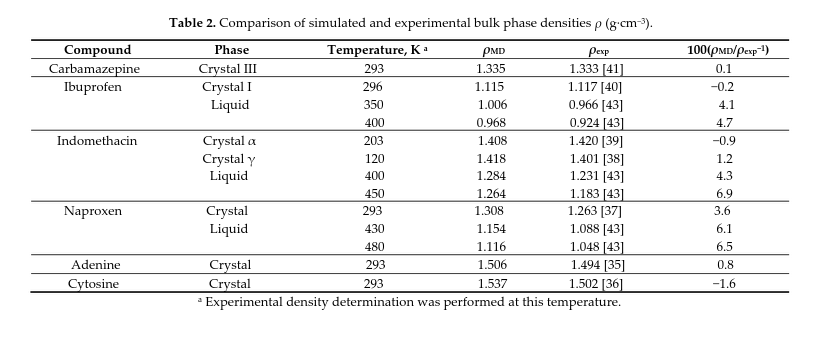
\includegraphics[width=1.0\linewidth]{img/tabulka_validace.png}
	\end{figure}

\subsubsection{Sulfathiazole FF parametrization}
A newly parametrized force field \cite{jorgensen_development_1996} was used for sulfathiazole. The charges on the atoms were calculated by quantum-chemical calculations using the Gaussian code \cite{frisch_gaussian16_2016}. At first, the structure was optimized using the B3LYP functional with the aug-cc-pVTZ basis set with the dispersion correction GD3BJ \cite{smith_revised_2016}. After finding the optimal geometric structure of the molecule, the charges on the atoms were fitted through the CHELPG (Charges from ELectrostatic Potentials using a Grid-based method) method and inserted into force field file.
 
The MD simulations of the sulfathiazole crystal were performed to validate the force field file parameters. The triclinic simulation box and barostat setting was used to account for the anisotropic character of the molecular crystal, other settings are similar to that with the PLA instead of calculating long-range interactions. The sulfathiazole crystal was simulated for three temperatures of 100, 200 and 300 K at 1 bar. The simulation results and experimental data obtained from literature \cite{drebushchak_crystal_2008} are given in the Table \ref{tab:sulfathiazol}.
 
    \begin{table}[htb]       
	\centering
	\begin{tabular}{lccc}
		\toprule
		Temperature, K & 100 & 200 & 300\\
		\midrule
		Experimental density $\rho_\mathrm{exp}$, g cm$^{-3}$  & $1.575 \pm 0.002$ & $1.560 \pm 0.002$ & $1.540 \pm 0.002$\\
		Calculated density $\rho_\mathrm{MD}$, g cm$^{-3}$ & $1.552 \pm 0.001$ & $1.534 \pm 0.002$ & $1.515 \pm 0.002$\\
		100($\rho_\mathrm{MD}/\rho_\mathrm{exp}-1$) & $-1.5$ & $-1.7$ & $-1.6$\\
		\midrule
		Experimental $\beta$ angle, $^{\circ}$ & $94.14$ & $93.905$ & $93.674$\\
		
		Calculated $\beta$ angle, $^{\circ}$ & $91.56$ & $91.64$ & $91.67$\\
		
		Calculated cell a length, \AA & 8.302 & 8.325 & 16.701\\
		
		Calculated cell b length, \AA & 8.236 & 8.275 & 16.625\\
		
		Calculated cell c length, \AA & 7.995 & 8.027 & 16.133\\
		\bottomrule
	\end{tabular}
	\caption{Comparison of simulated and experimental crystallographic parameters for sulfathiazole.}
	\label{tab:sulfathiazol}
\end{table}

There is a good match between the experimental and computed quantities. The relative deviations of experimental and calculated densities are very low. Other parameters do not indicate any notable deviations in the simulation box during the simulation, the crystallographic parameters of the unit cell are $a$ = 8.1896 \AA, $b$ = 8.532 \AA~and  $c$ = 15.447 \AA. 

\subsection{Simulations of mixtures of APIs and PLA}
\subsubsection{Calculated properties of mixtures}
Additive molar volumes ($V_{\text{m, mixing}})$ of the mixtures were evaluated from the simulations for each concentration using the Equation \ref{eq:VM}. For this reason, the average molar volumes of the simulation boxes were evaluated from simulations of pure API ($V_{\text{m}}^{\text{API}} $) and pure polymer ($V_{\text{m}}^{\text{PLA}}$) and from a mixture ($V_{\text{m}}^{\text{MIX}}$).

\begin{equation}\label{eq:VM}
	V_{\text{m, mixing}} = V_{\text{m}}^{\text{MIX}} - x_{\text{API}} V_{\text{m}}^{\text{API}} - x_{\text{PLA}} V_{\text{m}}^{\text{PLA}}
\end{equation}

Molar mixing energies were also evaluated in a similar way. The following Equation \ref{eq:EM} was used

\begin{equation}\label{eq:EM}
	E_{\text{m, mixing}} = E_{\text{m}}^{\text{MIX}} - x_{\text{API}} E_{\text{m}}^{\text{API}} - x_{\text{PLA}} E_{\text{m}}^{\text{PLA}},
\end{equation}

where $E_{\text{m}}^{\text{MIX}}$ is the average molar energy of the simulation box of the mixture, $E_{\text{m}}^{\text{API}}$ is the average molar energy of pure API, and $E_{\text{m}}^{\text{PLA}}$ is the averaged molar energy of pure PLA obtained from simulation. Mixing energies and volumes were calculated for all systems and both temperatures (300, 500~K), and the comparison is shown in Table \ref{tab:vobjemy}.  

\begin{table}[htb]
	\caption{Calculated mixing energies and volumes for API mixtures of different concentrations, simulations under 500 K.}
	\centering
	\begin{tabular}{lSSS} \toprule
		{\textbf{API}} & {\textbf{\boldmath{$x_{\text{API}}$}}} & \textbf{{\boldmath{$V_{\text{m, mixing}}$, cm$^3$/mol}}} & \textbf{{\boldmath{$E_{\text{m, mixing}}$, kJ/mol}}} \\
		\midrule
		carbamazepine  & 0.85 & 0.97 & 4.79 \\
		& 0.92 & 0.48 & 3.17 \\ 
		& 0.95   & 0.21 & 2.68    \\
		\midrule
		naproxen  & 0.85 & -7.07 & 7.50 \\
		& 0.92  & -8.50 & 6.24\\ 
		& 0.95   & -9.85 & 4.75   \\ 
		\midrule
		naproxen  & 0.85 & -7.07 & 7.50 \\
		& 0.92  & -8.50 & 6.24\\ 
		& 0.95   & -9.85 & 4.75   \\ 
		\midrule
		naproxen  & 0.85 & -7.07 & 7.50 \\
		& 0.92  & -8.50 & 6.24\\ 
		& 0.95   & -9.85 & 4.75   \\ 
		\bottomrule
	\end{tabular}
	\label{tab:vobjemy} 
\end{table}

The data show that a mixture of naproxen and PLA can create a more advantageous arrangement of molecules in space, meaning that the mixing volumes are negative. For carbamazepine the trend is the opposite; this could be caused by the shape of the carbamazepine molecule when the mixture needs more space. From the positive changes in energies, we can assume that mixing the APIs with PLA can reduce the interactions between API-API molecules, and also that new interactions between API and PLA are not developed in order to compensate for the API-API cohesion. 

\subsubsection{Glass transition temperature}
The glass transition temperatures of the mixtures were evaluated from the simulated annealing simulations by fitting a hyperbola to the temperature-density data. The whole methodology is described in the paper written by Alzate-Vargas\cite{alzate-vargas_uncertainties_2018}, the main equation of the fit is Equation \ref{eq:fit}

\begin{equation}\label{eq:fit}
	\rho(T)=\rho_0-a\left(T-T_0\right)-b\left[\frac{1}{2}\left(T-T_0\right)+\sqrt{\frac{\left(T-T_0\right)^2}{4}+e^c}\right].
\end{equation}

Since this method is sensitive to the initial state of the simulated box, more simulated data starting from different conformations must be provided to evaluate $T_\text{g}$. In this work we used 5 simulations from different initial states.

TO DO: DOPOČÍTAT PRO NOVÉ SIMULACE
The resulting value for carbamazepine is $T_{\text{g, cbz}} = 385 \pm 4$ (k = 2) and for naproxen is $T_{\text{g, nap}} = 365 \pm 2$ (k = 2). 

\subsubsection{Radial distribution functions}

Then, all RDFs of mixtures containing the API-API interaction were scaled onto the pure API RDF signal for better visualisation using the following Equation \ref{eq:RDF_formula}

\begin{equation}\label{eq:RDF_formula}
	\text{RDF}_{\text{scaled}} = \text{RDF} \cdot \frac{V_{\text{API}}}{N_{\text{API}}} \frac{N_{\text{mix}}}{V_{\text{mix}}},
\end{equation}

where $V_{\text{API}}$ is the average volume of the pure API simulation box, $N_{\text{API}}$ is the number of molecules in the pure API simulation box and, respectively, for mixtures.

Sampling the radial distribution function from the simulations was done to explore the interactions that are having the highest impact. The hydrogen bonds were mostly studied. All RDF data containing the API-API interaction in the mixtures were scaled for the intensities of the pure API signal. The strongest API-API interaction was chosen and plotted to study the change between simulations with different concentrations of PLA. 

For ibuprofen, the interaction between hydrogen from OH group and oxygen from OC was studied. For naproxen, the hydrogen bonding between two carboxyl groups was studied, for carbamazepine, hydrogen bonding was studied between the N$\text{H}_\text{2}$ and OC group and for indomethacine the interaction of oxygen from OC and hydrogen from OH was studied.  The selected atom types involved in interactions are visualised in the introduction section in Figure \ref{fig:APIs}. 

The RDF of the hydrogen bonding interaction of ibuprofen is shown in Figure \ref{fig:ibu_s_RDF_}.

\begin{figure}[htb!]
	\centering
	\subfloat{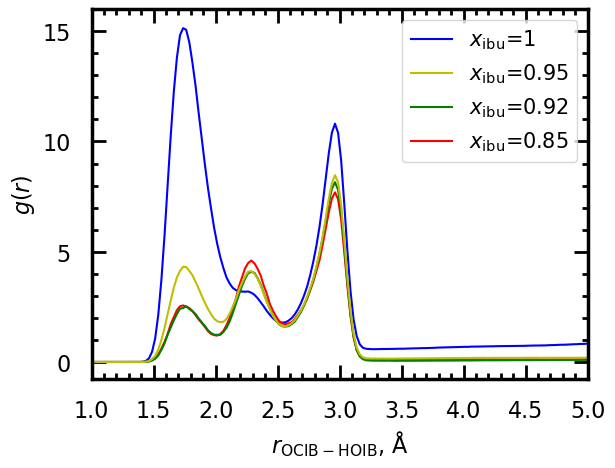
\includegraphics[width=0.4\linewidth]{img/rdf_ibu_s_api_r1.png}}\\
	%\subfloat{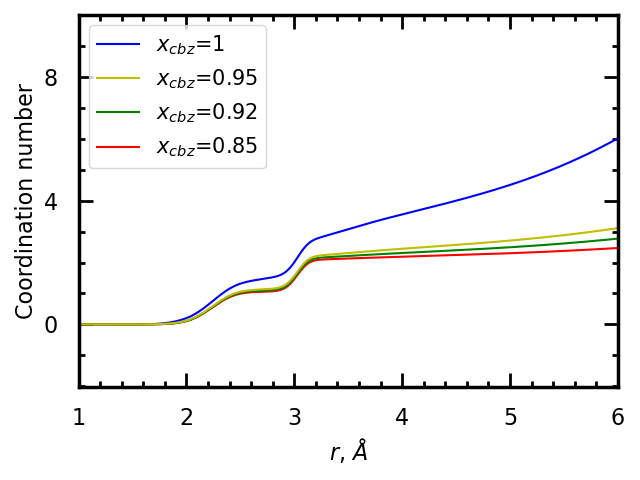
\includegraphics[width=0.4\linewidth]{img/coord_cbz_r2.png}} \\
	\subfloat{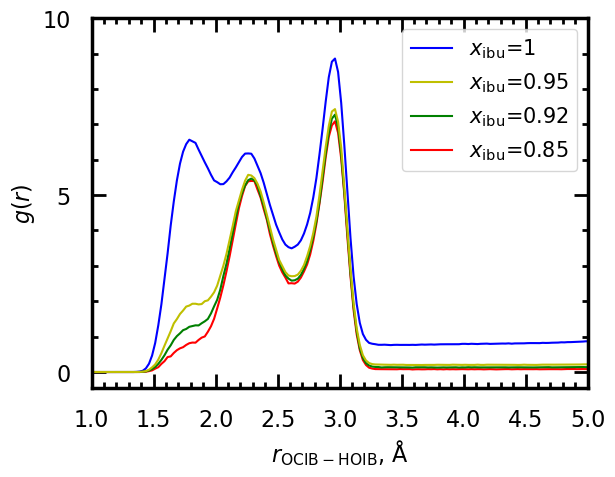
\includegraphics[width=0.4\linewidth]{img/rdf_ibu_s_api_r2.png}}
	%\subfloat{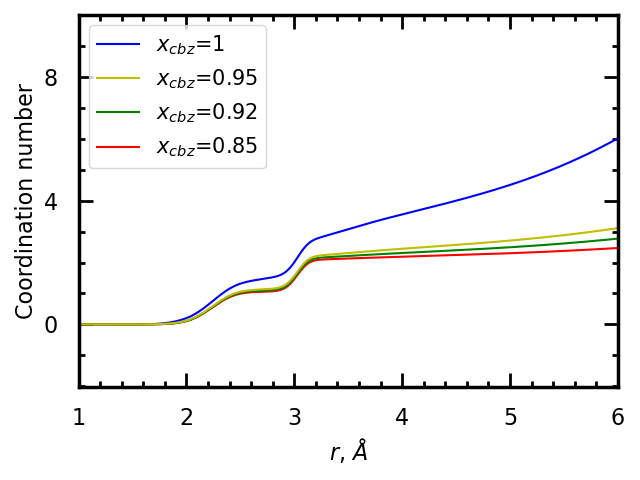
\includegraphics[width=0.4\linewidth]{img/coord_cbz_r2.png}}
	\caption{Radial distribution function of the API-API interaction between HOIB hydrogen atom bonded on oxygen and OCIB oxygen atom in a mixture of ibuprofen and PLA for different concentration normalized on values for pure ibuprofen, temperature of 300~K in the left upper corner and 500~K bottom left, coordination numbers on the right.}
	\label{fig:ibu_s_RDF_}
\end{figure}

The RDF of the selected interaction of naproxen is shown in Figure \ref{fig:nap_RDF_}. Here is the situation very different, the height of the first peak changes for different concentrations of PLA. For the higher concentration of PLA, the occurrence of the two hydrogen bonds carboxyl group contact is less important, and the contact of the groups is made only by one hydrogen bond.

\begin{figure}[htb!]
	\centering
	\subfloat{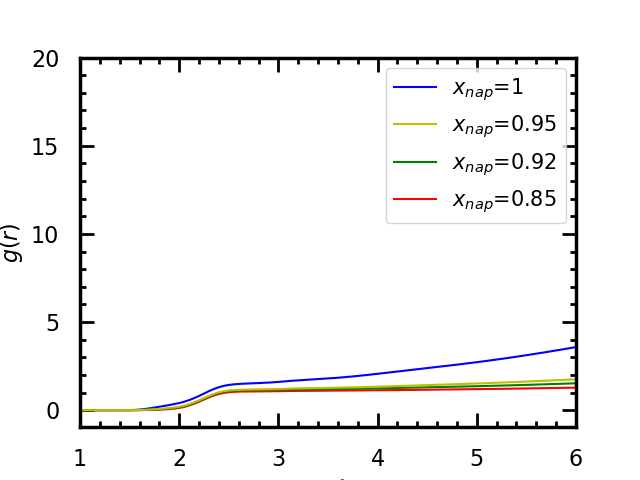
\includegraphics[width=0.4\linewidth]{img/rdf_nap_api_r1.png}}
	\subfloat{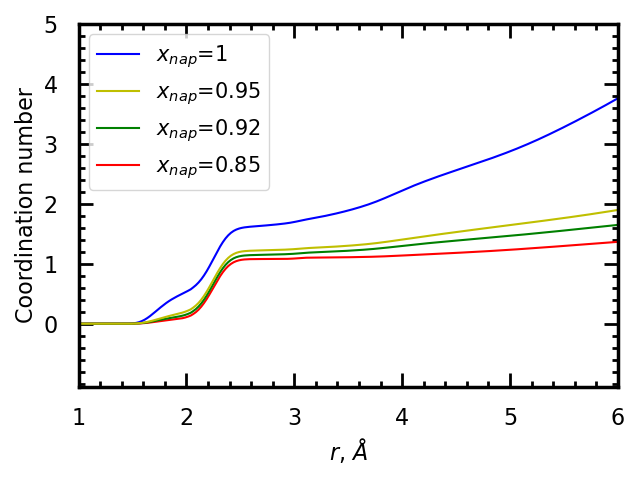
\includegraphics[width=0.4\linewidth]{img/coord_nap_r1.png}}\\
	\subfloat{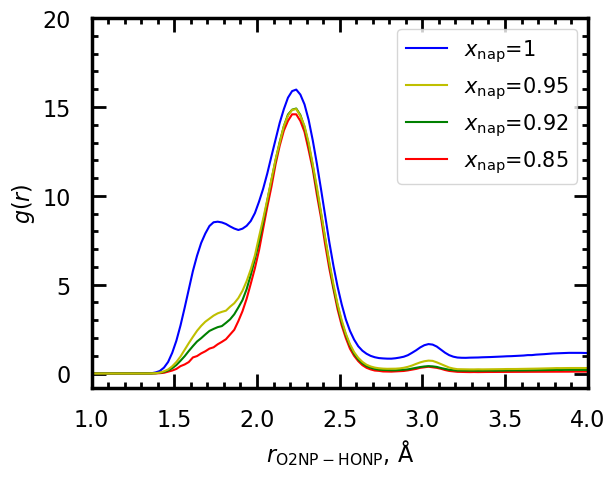
\includegraphics[width=0.4\linewidth]{img/rdf_nap_api_r2.png}}
	\subfloat{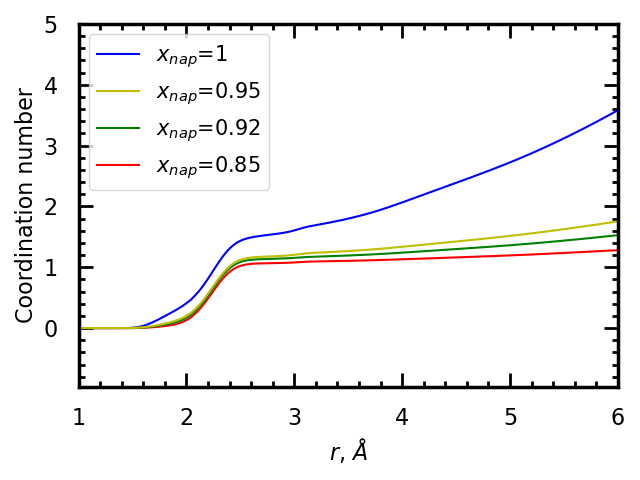
\includegraphics[width=0.4\linewidth]{img/coord_nap_r2.png}}
	\caption{Radial distribution function of the API-API interaction between HONP hydrogen atom and O2NP oxygen atom from COOH group in a mixture of naproxen and PLA for different concentration normalized on values for pure naproxen, temperature of 300~K in the left upper corner and 500~K bottom left, coordination numbers on the right.}
	\label{fig:nap_RDF_}
\end{figure}

The RDF of the hydrogen bonding interaction of carbamazepine is shown in Figure \ref{fig:cbz_RDF_}. The shape and signal response of the peaks for the mixtures are similar for both temperatures, meaning that the impact of the concentration of PLA on the cohesion of carbamazepine in the mixture is very low. 

\begin{figure}[htb!]
	\centering
	\subfloat{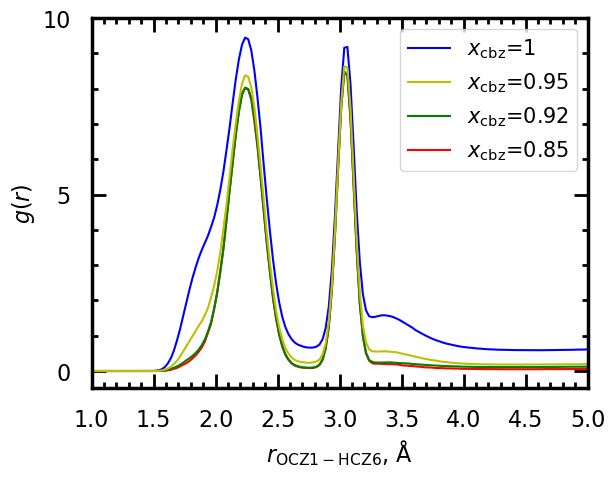
\includegraphics[width=0.4\linewidth]{img/rdf_cbz_api_r1.png}}
	\subfloat{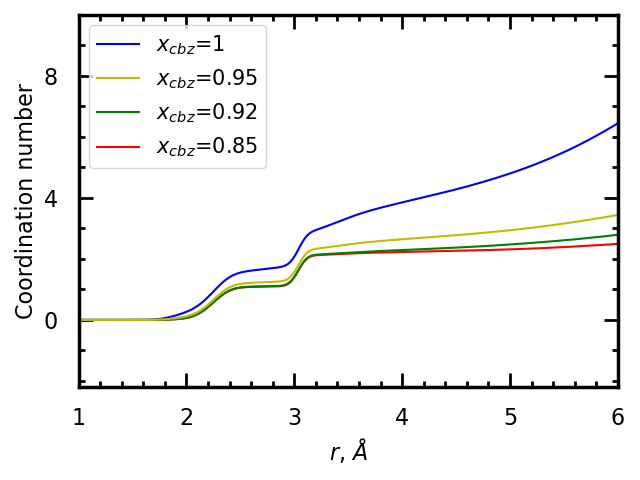
\includegraphics[width=0.4\linewidth]{img/coord_cbz_r1.png}}\\
	\subfloat{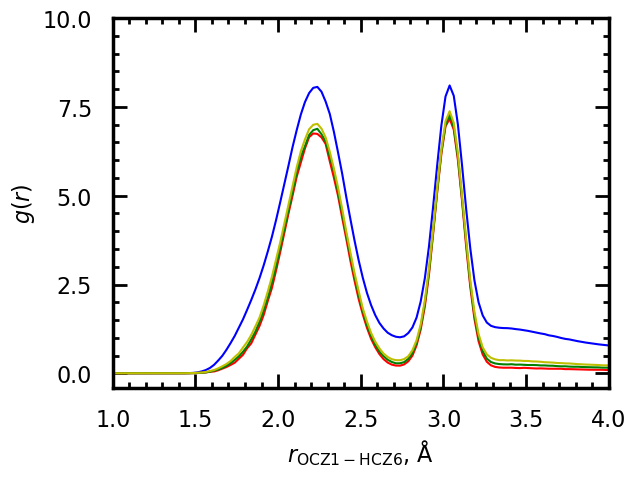
\includegraphics[width=0.4\linewidth]{img/rdf_cbz_api_r2.png}}
	\subfloat{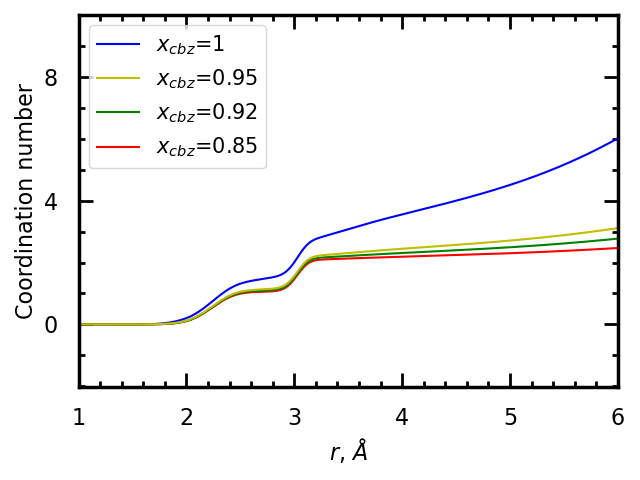
\includegraphics[width=0.4\linewidth]{img/coord_cbz_r2.png}}
	\caption{Radial distribution function of the API-API interaction between HCZ6 hydrogen atom bonded on nitrogen and OCZ1 oxygen atom in a mixture of carbamazepine and PLA for different concentration normalized on values for pure carbamazepine, temperature of 300~K in the left upper corner and 500~K bottom left, coordination numbers on the right.}
	\label{fig:cbz_RDF_}
\end{figure}

The RDF of the hydrogen bonding interaction of indomethacin is shown in Figure \ref{fig:indo_RDF_}.

\begin{figure}[htb!]
	\centering
	\subfloat{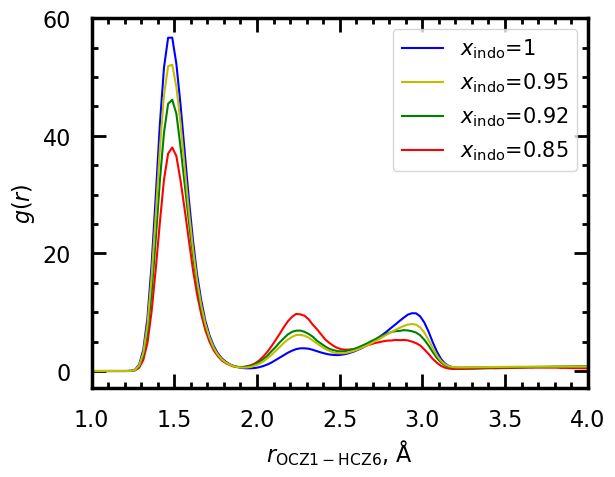
\includegraphics[width=0.4\linewidth]{img/rdf_indo_api_r1.png}}\\
	%\subfloat{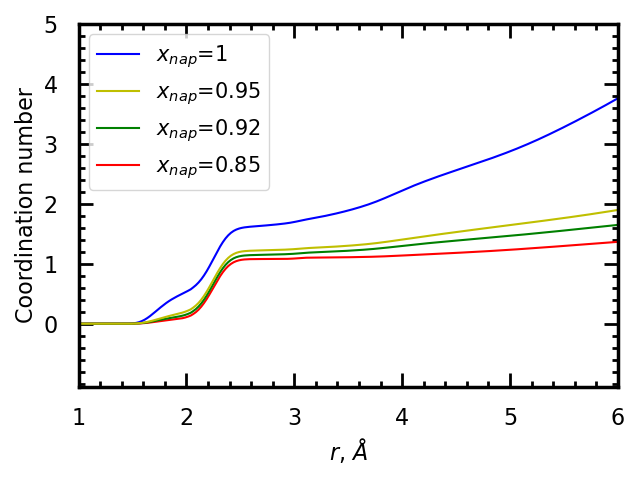
\includegraphics[width=0.4\linewidth]{img/coord_nap_r1.png}}\\
	\subfloat{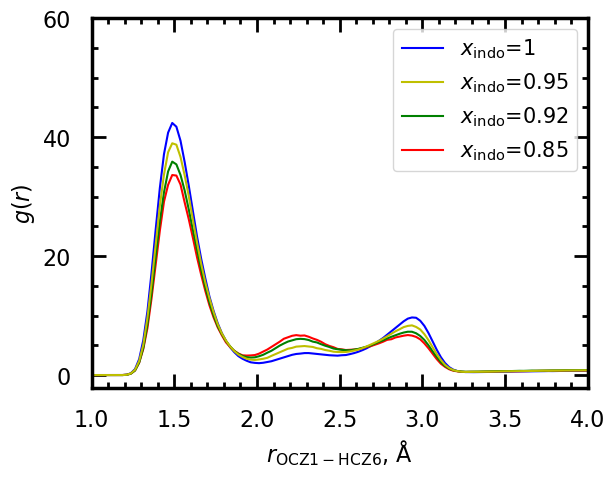
\includegraphics[width=0.4\linewidth]{img/rdf_indo_api_r2.png}}\\
	%\subfloat{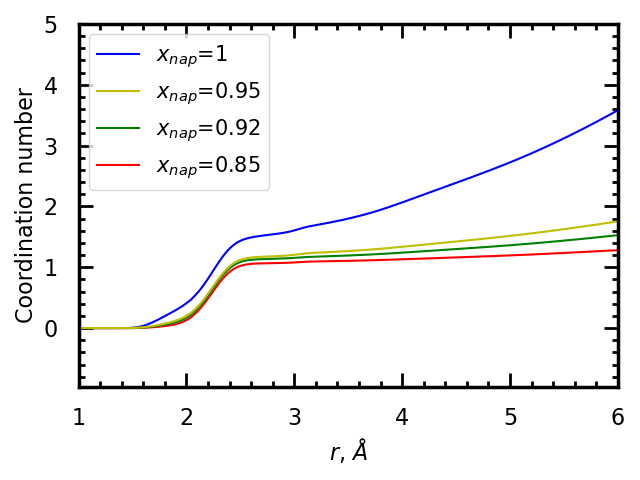
\includegraphics[width=0.4\linewidth]{img/coord_nap_r2.png}}
	\caption{Radial distribution function of the API-API interaction between HCZ6 hydrogen atom and OCZ1 oxygen atom from COOH group in a mixture of indomthacine and PLA for different concentration normalized on values for pure indomethacine, temperature of 300~K in the left upper corner and 500~K bottom left, coordination numbers on the right.}
	\label{fig:indo_RDF_}
\end{figure}




The hydrogen bonding between API and PLA was also studied. The contact visualization is available in Figure \ref{fig:contact}.

\begin{figure}[htb!]
	\begin{subfigure}{0.33\textwidth}
		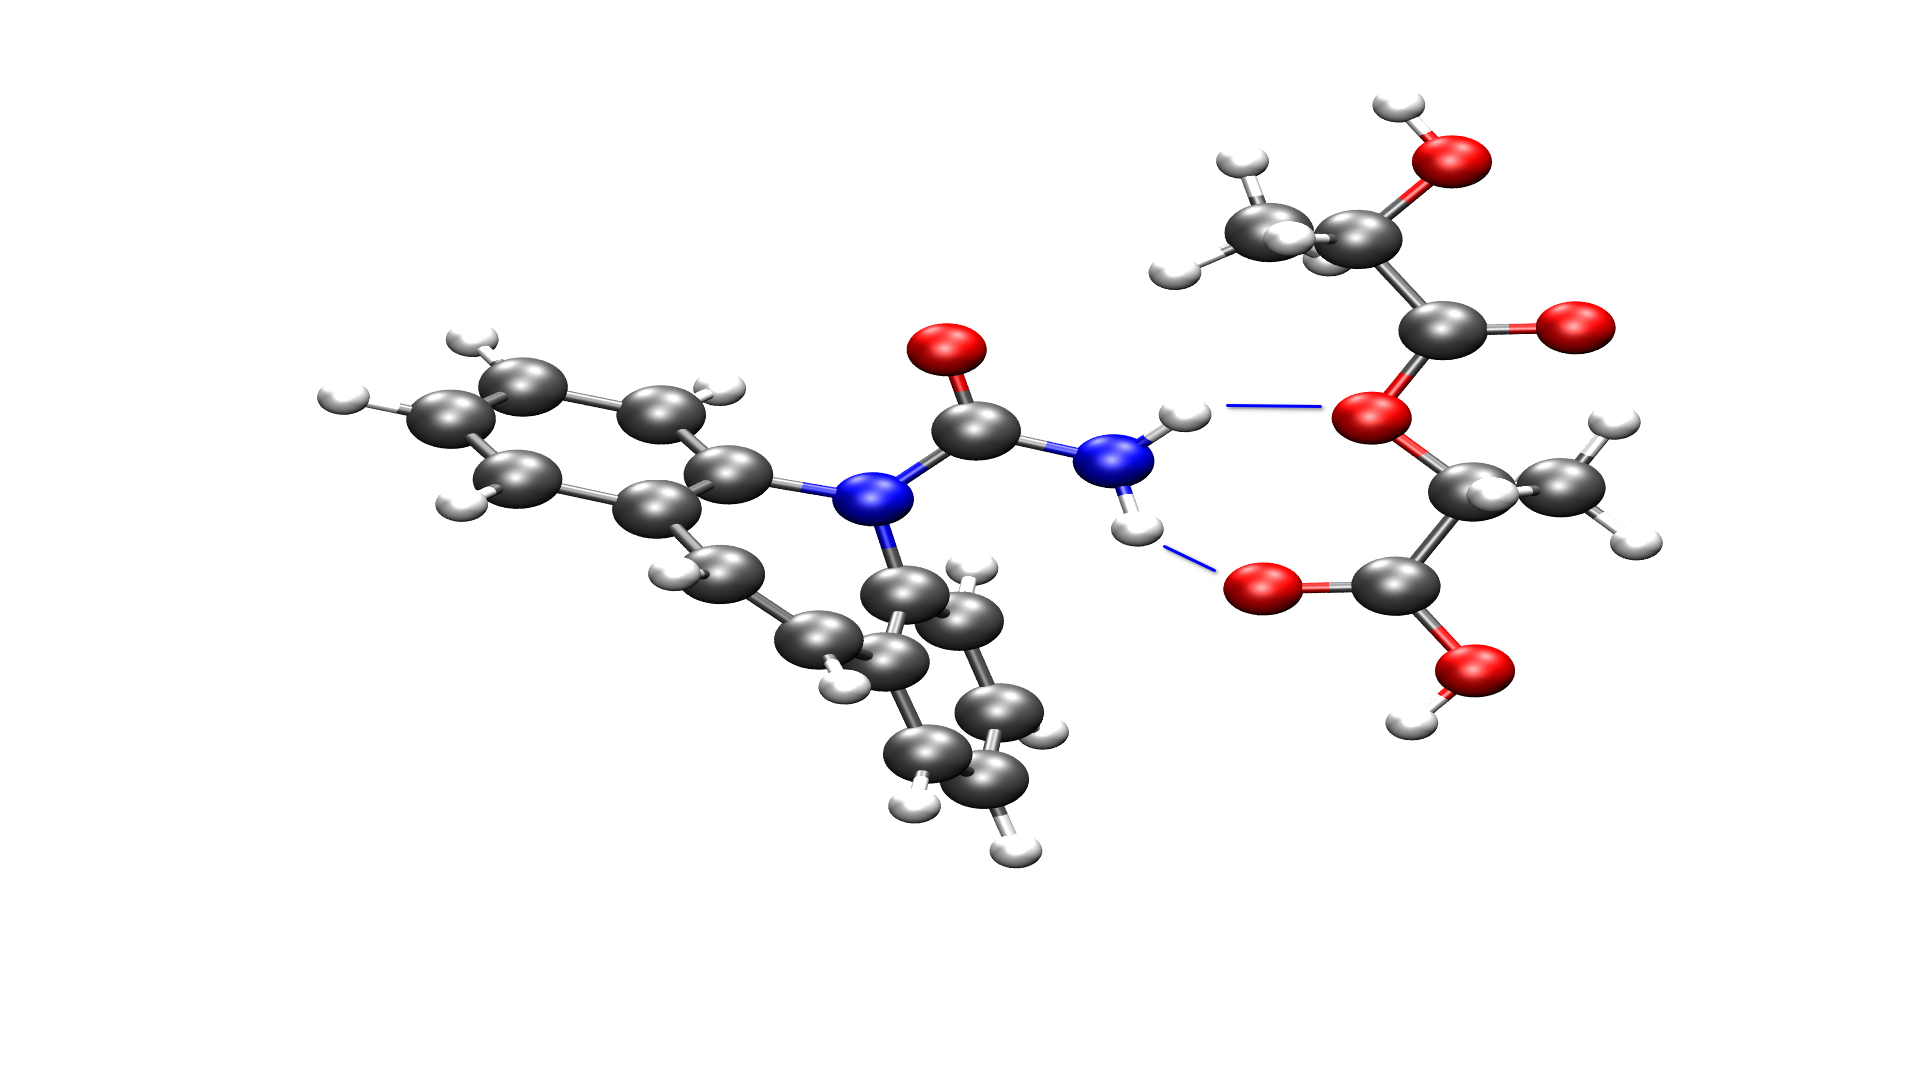
\includegraphics[width=\linewidth]{img/cbz_interakce.png} 
	\end{subfigure}
	\begin{subfigure}{0.31\textwidth}
		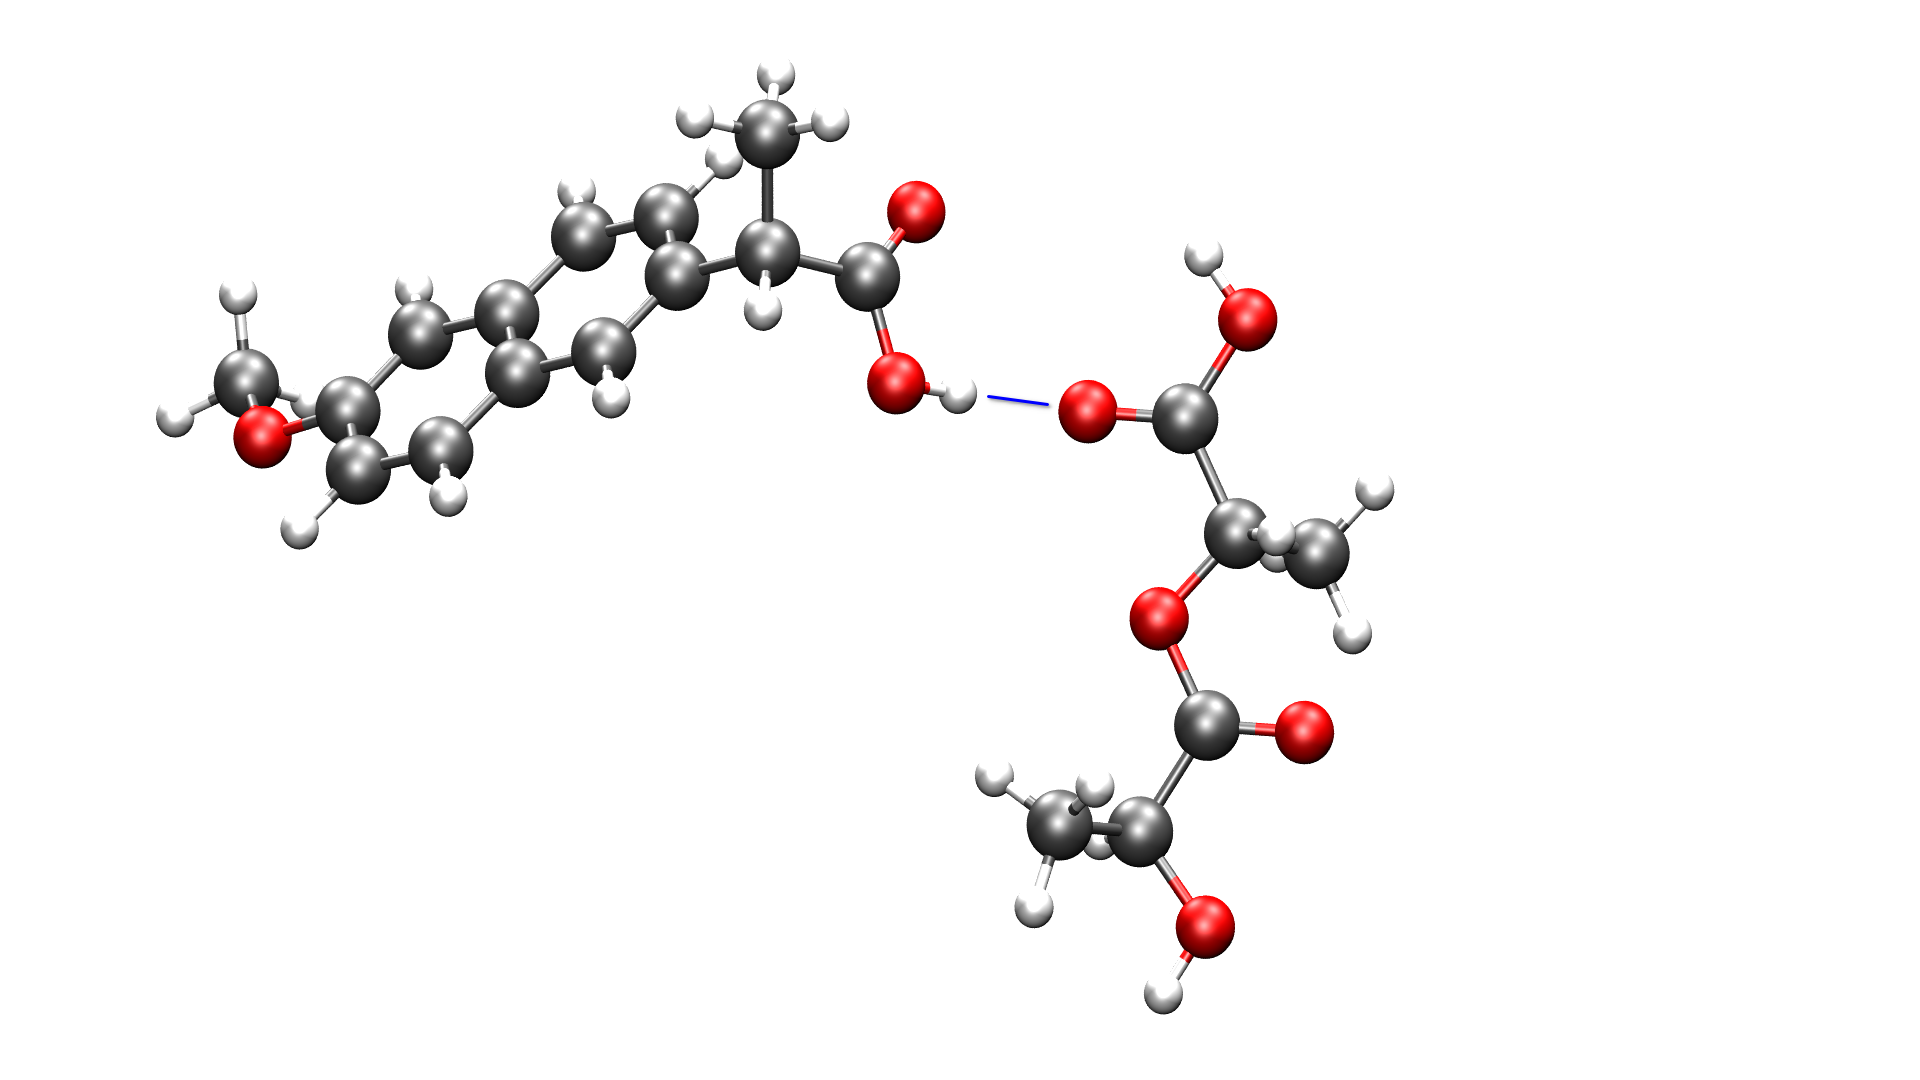
\includegraphics[width=\linewidth]{img/nap1_interakce.png} 
	\end{subfigure}   	
	\begin{subfigure}{0.33\textwidth}
		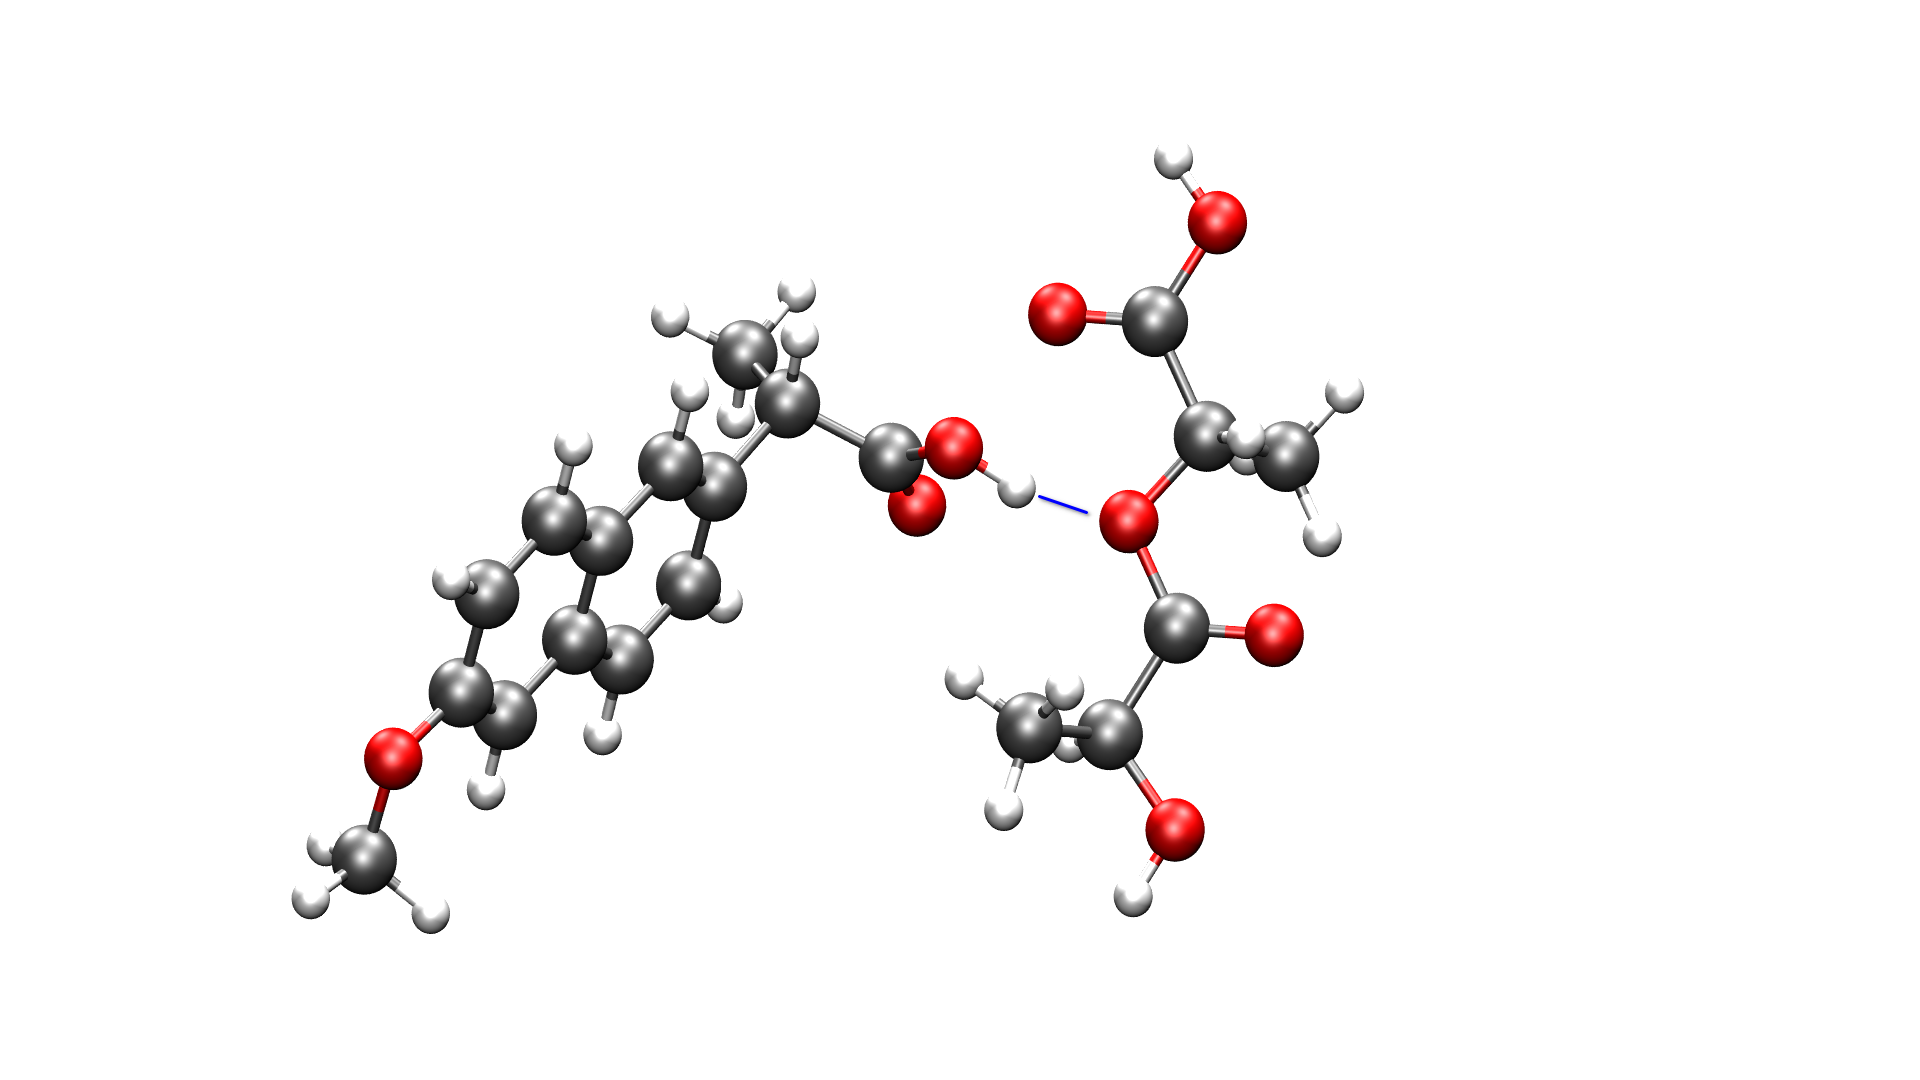
\includegraphics[width=\linewidth]{img/nap2_interakce.png} 
	\end{subfigure}
	\caption{Visualization of studied interactions of PLA-API, for carbamazepine on the left and for naproxen on the right.}
	\label{fig:contact}    
\end{figure}


The RDF of hydrogen bonding with the carbonyl group is shown in Figure \ref{fig:carbonyl}. For carbamazepine, those interactions are weak, we can see that the intensity of the first peak is really low. Under temperature 300 K slightly above one, but for 500 K the peak is below one, meaning that this interaction occurs less at a small distance than in the rest of the system. The value converges to one in a long distance. For naproxen, the interaction is more relevant, and the intensity of the peak is much higher but still less than in the NAP-NAP interactions.

The hydrogen bonds with the oxygen bonded by ether bond in PLA are shown in Figure \ref{fig:ether}. Here is the same situation as in the previous contact with carbonyl oxygen, but for naproxen, the interaction is less relevant. Both values also converge to 1 in a long distance.
\newpage
\begin{figure}[H]
	\centering
	\subfloat{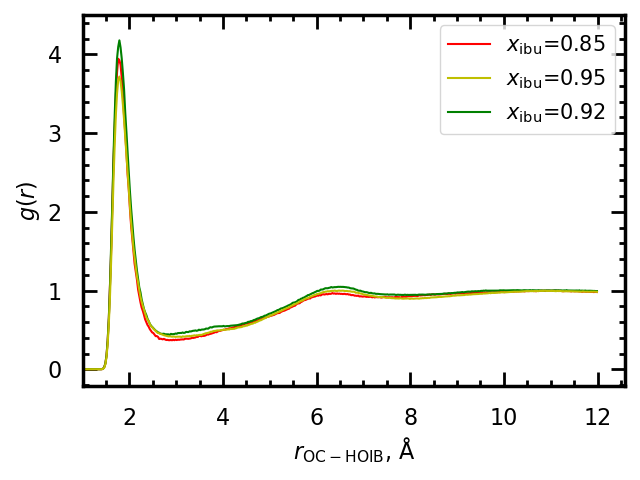
\includegraphics[width=0.5\linewidth]{img/RDF_ibu_s_20_2.png}}
	\subfloat{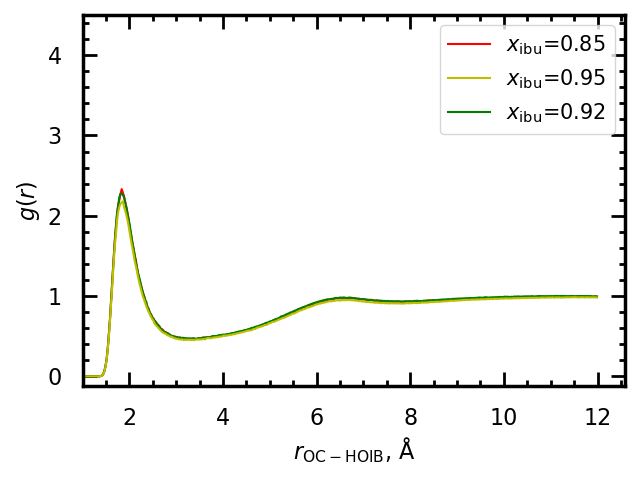
\includegraphics[width=0.5\linewidth]{img/RDF_ibu_s_20_2_r2.png}}\\
	\vspace{-0.2cm}
	\subfloat{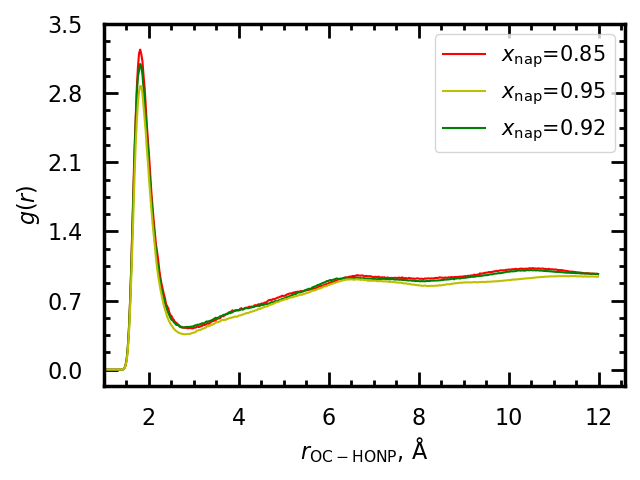
\includegraphics[width=0.5\linewidth]{img/RDF_nap_2_31.png}}
	\subfloat{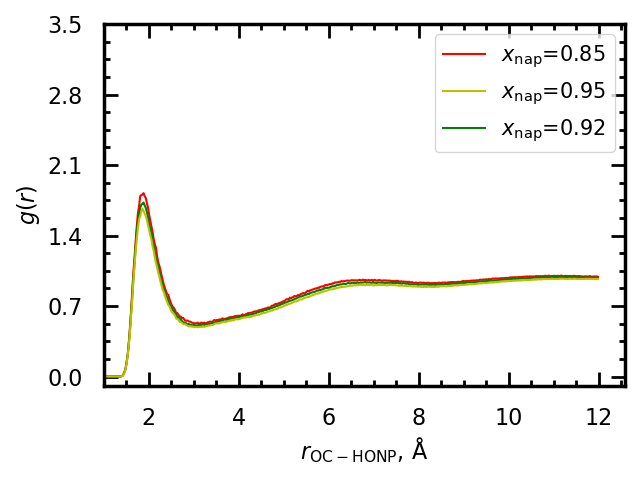
\includegraphics[width=0.5\linewidth]{img/RDF_nap_2_31_r2.png}}\\
	\vspace{-0.2cm}
	\subfloat{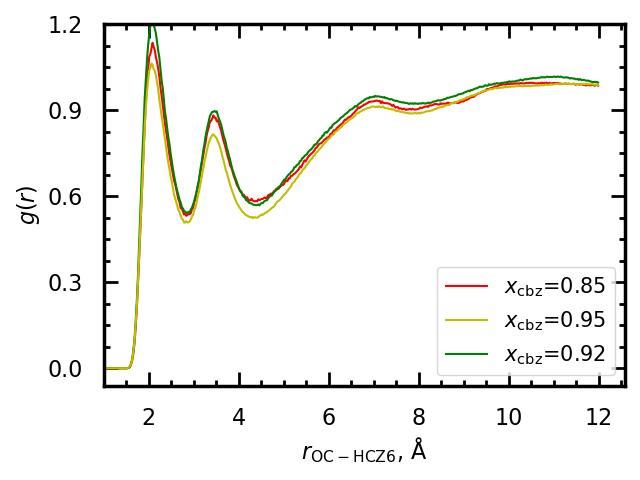
\includegraphics[width=0.5\linewidth]{img/RDF_cbz_2_27.png}}
	\subfloat{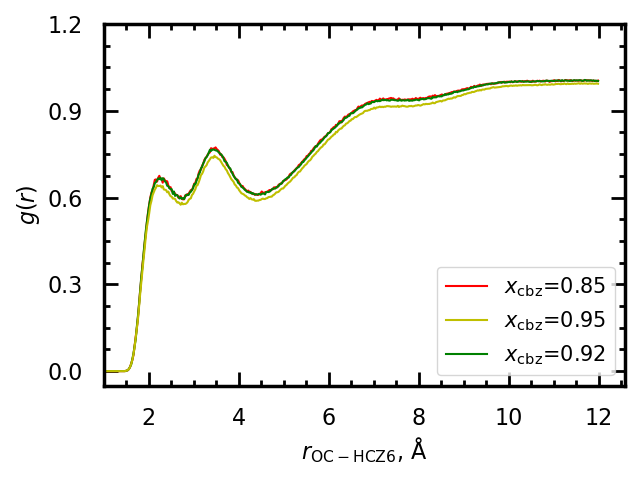
\includegraphics[width=0.5\linewidth]{img/RDF_cbz_2_27_r2.png}}\\
	\vspace{-0.2cm}
	\subfloat{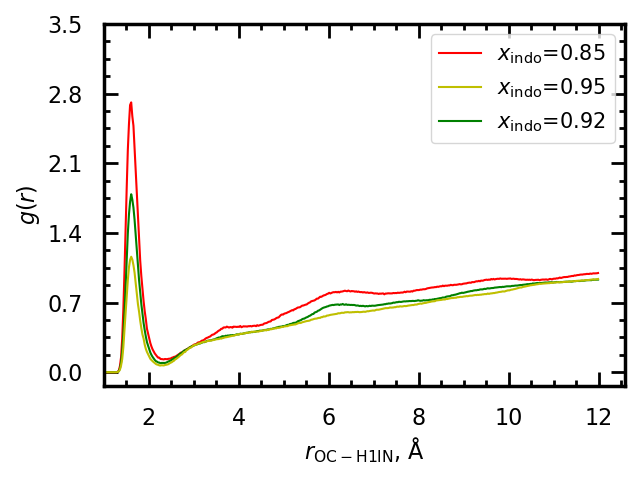
\includegraphics[width=0.5\linewidth]{img/RDF_indo_2_36.png}}
	\subfloat{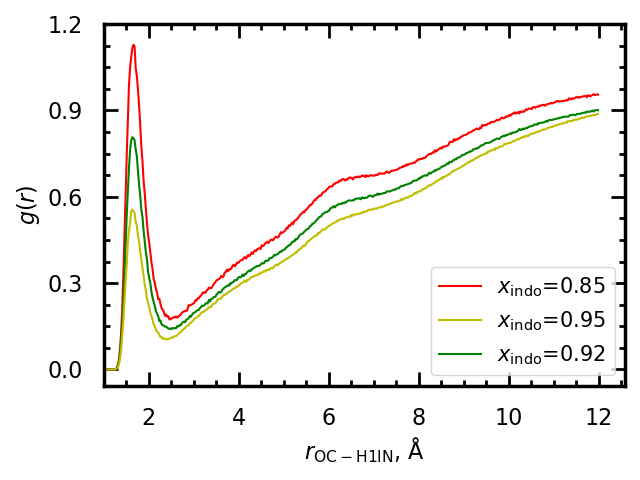
\includegraphics[width=0.5\linewidth]{img/RDF_indo_2_36_r2.png}}
		\vspace{-0.2cm}
	\caption{Radial distribution function of the interaction between hydrogen atoms and oxygen atom from carbonyl group in PLA, first ibuprofen on top, second naproxen, third carbamazepine and indomethacine in the bottom, temperature 300~K on the left and 500~K on the right.}
	\label{fig:carbonyl}
\end{figure}

\newpage
\begin{figure}[H]
	\centering
	\subfloat{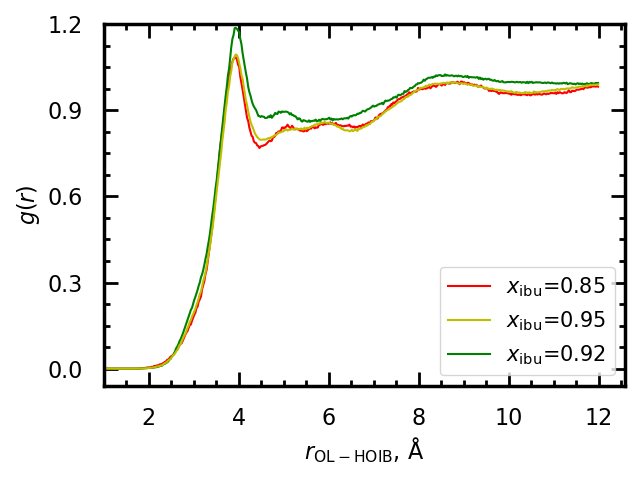
\includegraphics[width=0.5\linewidth]{img/RDF_ibu_s_20_6.png}}
	\subfloat{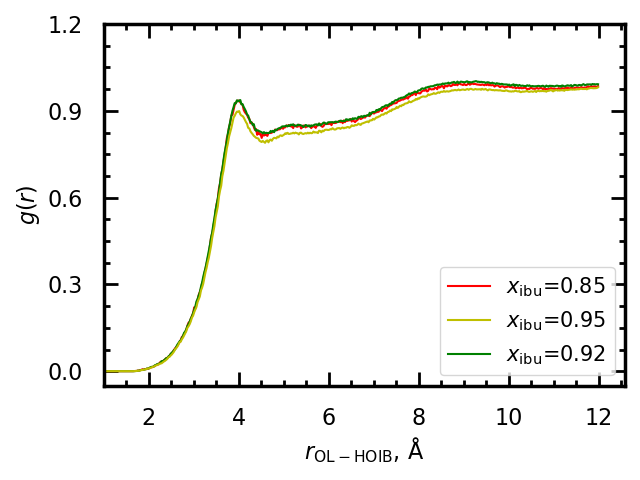
\includegraphics[width=0.5\linewidth]{img/RDF_ibu_s_20_6_r2.png}}\\
	\vspace{-0.2cm}
	\subfloat{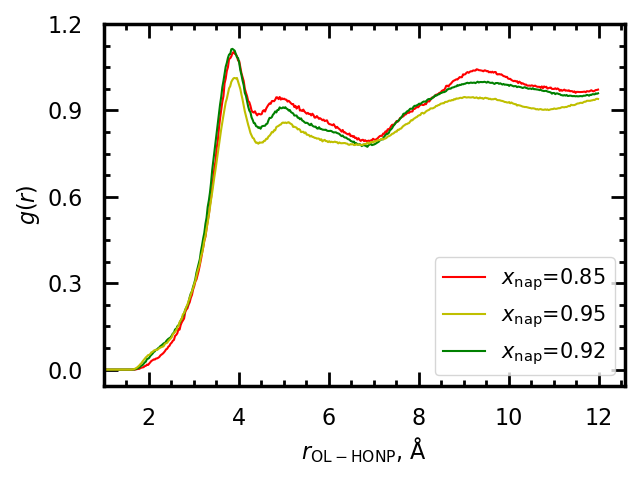
\includegraphics[width=0.5\linewidth]{img/RDF_nap_6_31.png}}
	\subfloat{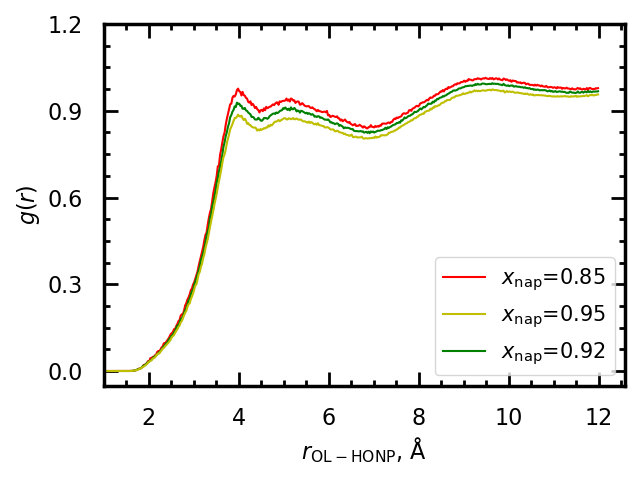
\includegraphics[width=0.5\linewidth]{img/RDF_nap_6_31_r2.png}}\\
	\vspace{-0.2cm}
	\subfloat{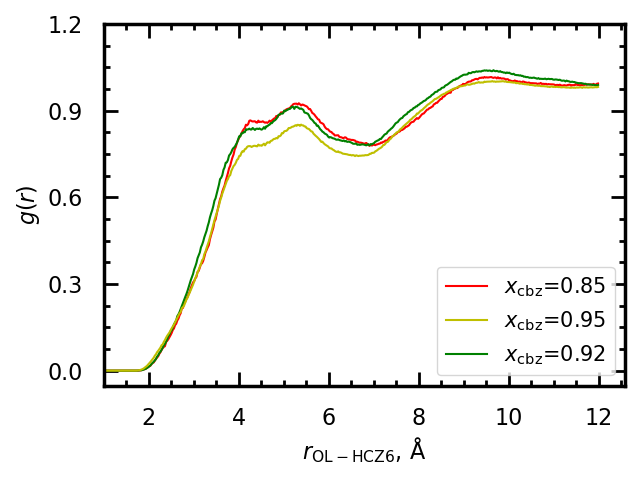
\includegraphics[width=0.5\linewidth]{img/RDF_cbz_6_27.png}}
	\subfloat{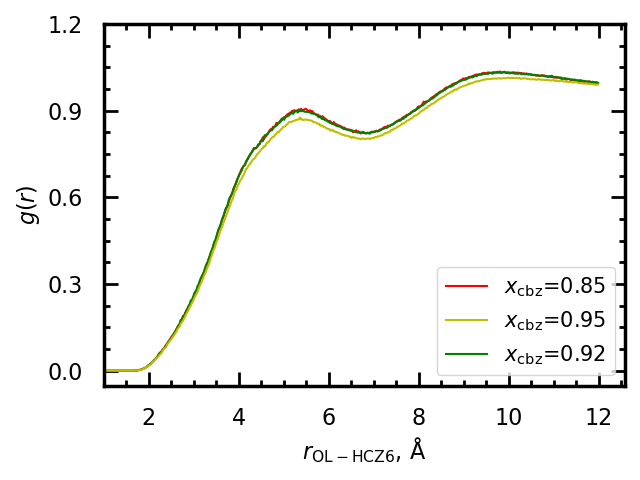
\includegraphics[width=0.5\linewidth]{img/RDF_cbz_6_27_r2.png}}\\
	\vspace{-0.2cm}
	\subfloat{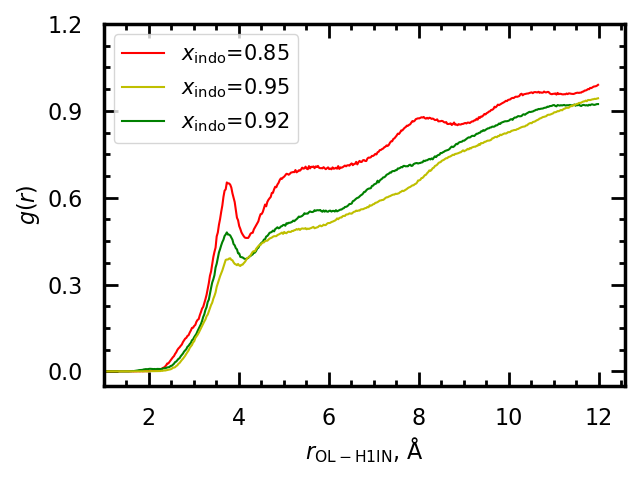
\includegraphics[width=0.5\linewidth]{img/RDF_indo_36_6.png}}
	\subfloat{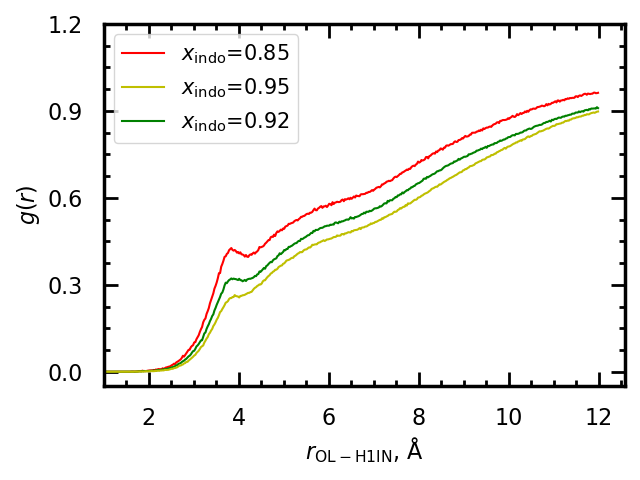
\includegraphics[width=0.5\linewidth]{img/RDF_indo_36_6_r2.png}}
	\vspace{-0.2cm}
	\caption{Radial distribution function of the interaction between hydrogen atoms and oxygen atom bonded by ether bond in PLA, first ibuprofen on top, second naproxen, third carbamazepine and indomethacine in the bottom, temperature 300~K on the left and 500~K on the right.}
	\label{fig:ether}
\end{figure}

\subsubsection{Diffusion coefficients}
The MSDs were sampled from the 10~ns long run simulations every 1000 fs (integration step 1 fs). At each sampled time step, obtained MSD data were averaged over all API molecules and then plotted as a function of simulation time. The MSD dependencies were then interpolated by a linear functions and related self-diffusivities of the API in the mixtures were evaluated from the slope of the line using the following Equation \ref{eq:D}

\begin{equation}\label{eq:D}
	D_{\text{API}} = \frac{a}{2d}, 
\end{equation}
where $D$ is the diffusion coefficient, $a$ is the slope of the line and $d$ is the dimensionality of the trajectory (3 in our case).

The MSD data for APIs in mixtures with PLA for $T$=500~K are plotted in Figure \ref{fig:msd_r2}. For ibuprofen, there is a significant difference between mobility of neat API and API mixed within the polymer. This could be result of very strong API-PLA interaction forming in the mixture. The data of carbamazepine shows that with increasing API concentration, mobility also increases. There is also not that enormous difference between neat API. For naproxen, it seems that there is no change for different concentrations of mixtures, also in neat API the mobility is higher. The situation for indometacine is completely different. For neat API the mobility is really low compared to mixtures with PLA. This behaviour seems strange, the reason could be, that in pure API, there are really strong API-API interactions that decrease the mobility. Also the MSD values are much lower.

\begin{figure}[htb]
	\centering
	\subfloat{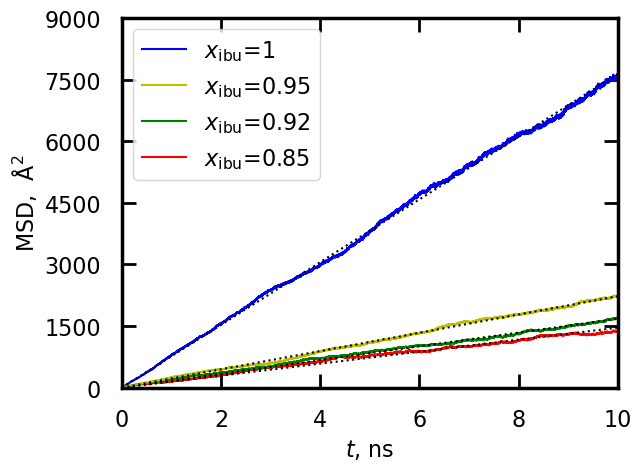
\includegraphics[width=0.4\linewidth]{img/msd_ibu_s_api_r2.png}}
	\subfloat{\includegraphics[width=0.4\linewidth]{img/msd_nap_api_r2.png}}\\
	\subfloat{\includegraphics[width=0.4\linewidth]{img/msd_cbz_api_r2.png}}
	\subfloat{\includegraphics[width=0.4\linewidth]{img/msd_indo_api_r2.png}} 
	\caption{MSD from simulations under 500 K, ibuprofen (\textbf{top left}), naproxen (\textbf{top right}), carbamazepine (\textbf{bottom left}) and indomethacin (\textbf{bottom right}).}
	\label{fig:msd_r2}    
\end{figure}

\newpage
Self-diffusivities were evaluated from the above data and plotted in Figure \ref{fig:d}. The data reveal that in pure liquid carbamazepine the diffusion is faster than in naproxen. For higher temperatures, the main factor affecting diffusion is the shape of the molecules, not the strength of the intermolecular interactions. This is caused because the kinetic energy is higher than the potential for higher temperatures.
\begin{figure}[htb!]
	\centering
	\includegraphics[width=0.4\linewidth]{img/d_coeficienty.png} 
	\caption{Self-diffusivities for carbamazepine and naproxen as a function of their concentration in the mixtures, temperature 500 K.}
	\label{fig:d}    
\end{figure}  

MSD was also evaluated at a lower temperature of 300 K, Figure \ref{fig:msd_r1}. There is the opposite trend. From these data sets, we can assume that carbamazepine has lower interactions with polymer because the mobility in the mixtures is higher than that in the pure state. The mobility of naproxen is always lower in mixtures, which is related to its stronger interactions with the polymer. The strength of the intermolecular interactions has a greater impact, meaning that paired molecules NAP-API slow the diffusion of other particles.

\begin{figure}[htb]
	\centering
	\subfloat{\includegraphics[width=0.4\linewidth]{img/msd_ibu_s_api_r1.png}}
	\subfloat{\includegraphics[width=0.4\linewidth]{img/msd_nap_api_r1.png}}\\
	\subfloat{\includegraphics[width=0.4\linewidth]{img/msd_cbz_api_r1.png}}
	\subfloat{\includegraphics[width=0.4\linewidth]{img/msd_indo_api_r1.png}} 
	\caption{MSD from simulations under 300 K, ibuprofen (\textbf{top left}), naproxen (\textbf{top right}), carbamazepine (\textbf{bottom left}) and indomethacin (\textbf{bottom right}).}
	\label{fig:msd_r1}    
\end{figure}


